\documentclass[11pt]{article}
\usepackage[margin=0.82in]{geometry}
\usepackage[T1]{fontenc}
\usepackage[utf8]{inputenc}
\usepackage{lmodern}
\usepackage{microtype}
\usepackage{graphicx}
\usepackage{booktabs}
\usepackage{longtable}
\usepackage{tabularx}
\usepackage{array}
\usepackage{amsmath,amssymb}
\usepackage{enumitem}
\usepackage{caption}
\usepackage{subcaption}
\usepackage{float}
\usepackage{xcolor}
\usepackage{hyperref}
\usepackage{url}
\usepackage{fancyhdr}
\usepackage{natbib}
\usepackage{listings}
\usepackage{tcolorbox}

\definecolor{navy}{HTML}{284B63}
\definecolor{rust}{HTML}{B85C38}
\definecolor{green}{HTML}{4F8A5B}
\definecolor{light}{HTML}{F4F7F8}
\hypersetup{colorlinks=true,linkcolor=navy,citecolor=green,urlcolor=rust,pdftitle={Beyond a Perfect Score},pdfauthor={Mame Diarra Toure and Bonaventure F. P. Dossou}}
\pagestyle{fancy}
\fancyhf{}
\lhead{Rare Disease, Real Kid: MVA Hackathon 2026}
\rhead{Track 1 methods and generalization report}
\cfoot{\thepage}
\setlength{\headheight}{14pt}
\setlist{nosep,leftmargin=*}
\setlist[description]{leftmargin=0pt,labelindent=0pt,labelsep=0.6em}
\setlength{\parindent}{0pt}
\setlength{\parskip}{0.55em}
\newcolumntype{Y}{>{\raggedright\arraybackslash}X}
\newcommand{\good}[1]{\textcolor{green}{\textbf{#1}}}
\newcommand{\warn}[1]{\textcolor{rust}{\textbf{#1}}}
\newcommand{\code}[1]{\texttt{#1}}
\newcommand{\pp}{percentage points}
\lstset{basicstyle=\ttfamily\small,breaklines=true,frame=single,backgroundcolor=\color{light},columns=fullflexible}

\title{\textbf{Beyond a Perfect Score}\\[0.35em]
\large Genome-wide diagnosis, Bayesian variant ranking, uncertainty, and temporal generalization for the Rare Disease, Real Kid MVA Hackathon 2026}
\author{\href{https://arradiat.github.io}{Mame Diarra Toure} \& \href{https://bonaventuredossou.github.io}{Bonaventure F. P. Dossou}\\[0.3em]\small Research lead, Bayesian modeling and generalization analysis}
\date{7 September 2026}

\begin{document}
\maketitle

\begin{tcolorbox}[colback=light,colframe=navy,title=TL;DR]
The genome-wide pipeline identified the accepted compound-heterozygous \textit{BUB1B} pair at rank 1, and every transferred model reproduced the maximum Track 1 score; the work that distinguishes this submission is the evidence trail explaining why the pair is credible, where the models generalize, where Bayesian uncertainty helps.
\end{tcolorbox}

\begin{abstract}
Track 1 of the Rare Disease, Real Kid Hackathon asks participants to identify the causal variant or variant pair in one child with mosaic variegated aneuploidy (MVA). We developped a genome-wide workflow and processed the gated whole-genome data, aligned more than one billion reads, normalized and phased 5.08 million variants, joined functional annotations to all but one heterozygous allele, and ranked a compound-heterozygous \textit{BUB1B} hypothesis first. The uploaded prediction received 100 Rank Points and F-max 1.0. We then asked a harder question: can a learned method reproduce the child-level result and transfer to variants and patients unavailable at training time?

We evaluated a linear Bayesian ranker, deterministic gradient boosting and neural networks, a five-network deep ensemble, low-rank singular Bayesian neural networks (SBNNs), full-weight Bayes-by-Backprop (BBB) networks, wider Bayesian architectures, and a validation-selected consensus. All challenge adapters placed the accepted pair first and achieved the same perfect Track 1 score. Perfect agreement on one proband did not distinguish the models. On an untouched temporal ClinVar holdout, the wide rank-50 SBNN achieved the best simulated top-1 ranking (84.35\%) and F-max (0.9235), while the deep ensemble remained the best detector of unseen genes (OOD AUROC 0.7485). On 719 post-2023 solved Phenopacket hypotheses, molecular-only top-1 accuracy was about 34\%; an HPO-conditioned dense BBB reached 58.9\% $\pm$ 1.0\% across five resampled candidate cohorts. The best result on 64 two-variant cases was 68.1\% top-1. These patient tests use compact ClinVar-derived candidate sets, not complete external exomes, so they support transfer of the ranking function but not a clinical diagnostic sensitivity claim.

The contribution is therefore a reproducible methodology with explicit separation of candidate generation from ranking, strict temporal and gene-aware evaluation, calibrated claims about uncertainty, attribution of upstream data and features, and a clear path to full patient-level validation through PhEval.
\end{abstract}
\section{Introduction}
\subsection{The pipeline}

Figure~\ref{fig:system} is the project pipeline. The first two stages establish a valid patient-specific candidate universe. The learned models then estimate molecular pathogenicity, an uncertainty layer flags cases unlike the training evidence, and phenotype plus inheritance logic returns the analysis to the patient rather than treating isolated variants as the endpoint.

\begin{figure}[H]
\centering
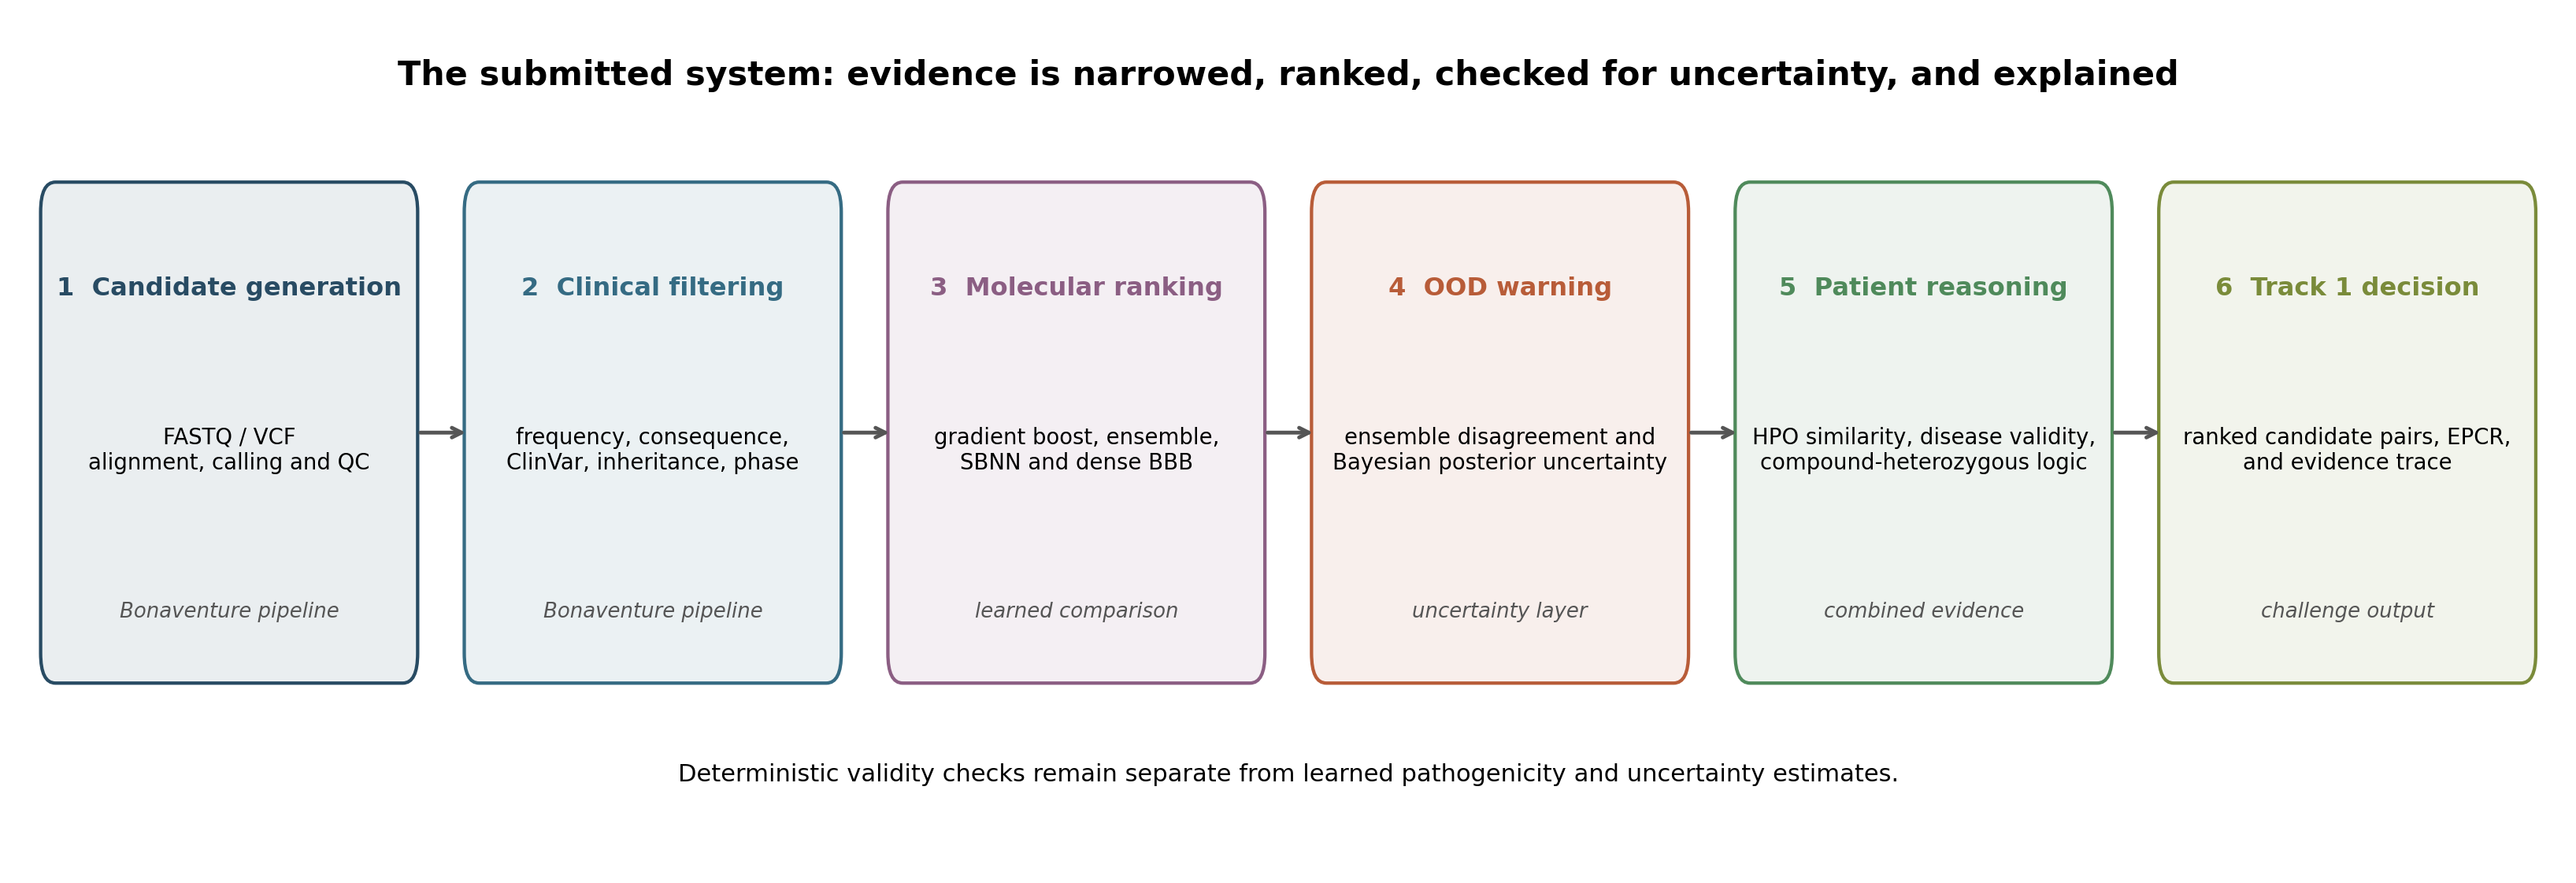
\includegraphics[width=\textwidth]{figures/system_pipeline.png}
\caption{The complete Track 1 system. The pipeline supplies candidate generation and clinical filtering. The comparative modeling work supplies molecular ranking and uncertainty. Patient-level reasoning combines those outputs with HPO similarity, disease validity, phase, and compound-heterozygous logic. The final product is a ranked pair and an inspectable evidence trace.}
\label{fig:system}
\end{figure}

For the submitted child, this chain reduces 5.08 million variants to six reportable pairs and ranks the accepted \textit{BUB1B} pair first. For external evaluation, candidate generation is held fixed and the ranking layers are tested on temporal ClinVar variants and later solved Phenopacket cases. That separation makes the scope of each result clear: the child score evaluates the full system on one proband, while the external benchmarks test transfer of the molecular and phenotype-ranking components.
\subsection{The argument}

The report follows one claim from raw observations to its limits. We begin with the child's genome and phenotype, align the reads, check the reference representation, normalizes and annotates millions of variants, phase the heterozygous calls, apply genotype and inheritance filters, construct same-gene pairs, and only then produces the candidate table. This is the end-to-end diagnostic path that leads to \textit{BUB1B}.

The leading pair is then justified biologically. One allele is a pathogenic stop-gain. The second is an ultra-rare missense allele with strong sequence quality and computational support but unresolved clinical significance. Both are required by the compound-heterozygous hypothesis, direct cis pairs are excluded, the MVA phenotype is consistent with biallelic \textit{BUB1B} dysfunction, and the remaining phase uncertainty is reported rather than hidden.

The learned comparison is deliberately downstream of those validity checks. No model input contains the accepted rank, the challenge answer, or a \textit{BUB1B}/MVA bonus. The temporal adapter also excludes clinical significance, submitted scores, and unavailable patient predictors when these would leak the answer. The report compares deterministic gradient boosting, a dense neural network, a five-network ensemble, a linear Bayesian ranker, low-rank SBNNs, dense BBB networks, wider Bayesian models, and a validation-selected consensus under shared evaluation rules.

The child result alone cannot establish generalization, even though every compatible model reproduces the maximum score. Generalization is therefore tested separately with a 2023-to-2026 ClinVar split, gene-disjoint validation, an untouched odd-ID holdout, and 719 post-2023 solved Phenopacket cases. These experiments show useful transfer, particularly after HPO conditioning, but also show a sharp known-gene versus unseen-gene gap.

Uncertainty is treated as a referral signal, not as a decorative Bayesian output. NLL, Brier score, ECE, posterior or ensemble disagreement, unseen-gene OOD AUROC, and selective prediction are examined separately from ranking accuracy. The ensemble currently gives the clearest unfamiliar-gene warning, while the wide rank-50 SBNN gives the best temporal ranking. A practical pipeline should use that warning to send unfamiliar or unstable cases for review rather than allowing a confident-looking score to close the case automatically.

The scope of the claim stays narrow. The external benchmark evaluates molecular pathogenicity and candidate ranking in constructed candidate sets. It does not measure recall from complete genomes, prove the two child alleles are in trans, establish the missense allele functionally, or demonstrate clinical probability calibration. A full VCF-based PhEval experiment is the next test required for a true multi-patient end-to-end diagnostic claim.
\section{The challenge and its evaluation}

\subsection{Two tracks, two different scientific tasks}

The challenge uses real genomic and clinical data from a child diagnosed with MVA. The gated repository contains approximately 85~GB across 11 files and recommends 100--150~GB of working storage because alignment, indexes, and intermediate files are larger than the compressed download \citep{hackathondata2026}. The submission period runs from 24 August to 24 October 2026.

Track 1 asks for a ranked list of primary causal variants or compound-heterozygous pairs. Its automated metrics are Rank Points and F-max. A methods report is mandatory but judged qualitatively. Track 2 asks for a mechanism-based drug-repurposing proposal and is panel-scored for scientific rigor (35\%), potential impact (25\%), innovation (25\%), and scalability (15\%) \citep{hackathon2026}.

\subsection{What Rank Points and F-max measure}

Let the accepted causal allele set for a proband be $G$ and the allele set in submitted row $i$ be $S_i$. The full-match rank is the first row for which $S_i=G$. Rank Points are a decreasing function of that rank, with rank 1 receiving 100 points. Partial credit is possible when only one allele of a compound-heterozygous answer is recovered.

Each row also contains an estimated probability of causal relationship (EPCR). For every submitted threshold $t$, the evaluator retains rows with EPCR at least $t$, converts them to predicted alleles, and computes
\begin{equation}
P(t)=\frac{TP(t)}{TP(t)+FP(t)},\qquad
R(t)=\frac{TP(t)}{TP(t)+FN(t)},
\end{equation}
\begin{equation}
F_1(t)=\frac{2P(t)R(t)}{P(t)+R(t)},\qquad
F_{\max}=\max_t F_1(t).
\end{equation}
On one solved proband, $F_{\max}=1$ is possible whenever a threshold isolates exactly the accepted pair. It does not establish probability calibration across patients. This distinction becomes important because our perfect models assign the top pair EPCR values ranging from roughly 0.35 to 0.95.
\section{Biology Primer}

\subsection{Variants, alleles, genes, and inheritance}

A variant is a difference between the child's DNA and a reference genome. Humans usually carry two copies of each autosomal gene, one inherited from each parent. A heterozygous variant is present on only one copy. In a recessive disorder, one damaging allele is often insufficient; both copies must be affected.

A \emph{compound-heterozygous} hypothesis contains two different damaging variants in the same gene. For the hypothesis to be recessive, the variants should be in \emph{trans}, meaning they lie on different parental copies. If they are in \emph{cis}, both lie on the same copy and the other copy may remain functional. Short reads cannot always phase variants separated by many kilobases, so ``phase unknown'' is uncertainty, not evidence for cis.

\subsection{Mosaic variegated aneuploidy and \textit{BUB1B}}

MVA is a rare chromosome-instability syndrome in which different cells carry different chromosome gains or losses. It can involve growth restriction, microcephaly, developmental abnormalities, and increased cancer risk. Biallelic pathogenic variants in \textit{BUB1B} are an established cause \citep{bub1b2004}.

\textit{BUB1B} encodes BUBR1, a core spindle-assembly-checkpoint protein. During cell division, the checkpoint delays chromosome separation until chromosomes are properly attached to the mitotic spindle. Reduced BUBR1 function allows segregation errors, providing a direct mechanistic bridge from genotype to aneuploid cells and cancer susceptibility \citep{bub1bmechanism2010}.
The Human Phenotype Ontology (HPO) assigns standardized identifiers to clinical findings \citep{hpo2021}. A patient is represented by a set of observed and sometimes explicitly absent HPO terms. Phenotype matching asks whether diseases associated with a candidate gene explain that set. It is not a substitute for molecular evidence. A gene can match the phenotype while the patient's variants in that gene are benign; conversely, a genuinely novel disease gene may have no prior phenotype annotation.

\section{Clinical phenotype and target hypothesis}

The supplied phenotype included rhabdomyosarcoma (HP:0002859), nephrocalcinosis (HP:0000121), short stature (HP:0004322), failure to thrive (HP:0001508), skeletal muscle atrophy or low muscle mass (HP:0003202), premature birth (HP:0001622), severe intrauterine growth restriction or small-for-gestational-age birth (HP:0001518), and parental recurrent spontaneous abortion (HP:0200067).

The genome-wide analysis ranked the following pair first:

\begin{table}[H]
\centering
\caption{Leading \textit{BUB1B} hypothesis on GRCh38.}
\small
\begin{tabularx}{\textwidth}{p{0.17\textwidth}p{0.16\textwidth}p{0.25\textwidth}Y}
\toprule
Variant & Protein consequence & Population evidence & Interpretation \\
\midrule
chr15:40209701 T$>$G & p.Leu737Ter & gnomAD v4.1.1 AF $7.4\times10^{-5}$; no homozygotes & Stop-gain; ClinVar pathogenic/likely pathogenic, two stars; CADD PHRED 38; LOFTEE high-confidence loss of function. \\
chr15:40220612 T$>$G & p.Asn1002Lys & One allele among 1,614,226; AF $6.2\times10^{-7}$; no homozygotes & Rare missense; CADD 26.4, REVEL 0.472, PolyPhen 0.997. This nucleotide change has no ClinVar record; the same amino-acid substitution produced by another nucleotide change is a VUS. \\
\bottomrule
\end{tabularx}
\end{table}

The first allele is a strong pathogenic anchor. The second is the key uncertainty. Its rarity, sequence quality, phenotype context, and occurrence with a pathogenic allele support the pair, but computational scores do not establish pathogenicity. The variants are 10,911 bases apart and were not connected by a short-read phase block. Parental sequencing, long-range phasing, or a functional assay would materially strengthen the conclusion.
\section{Data provenance, access, and storage decisions}

\subsection{Training Data for Uncertainty-Aware models}

\footnotesize
\begin{longtable}{p{0.16\textwidth}p{0.17\textwidth}p{0.24\textwidth}p{0.29\textwidth}}
\caption{Data provenance and role in the project.}\\
\toprule
Dataset & Source and access & Local acquisition & Use and boundary \\
\midrule
\endfirsthead
\toprule
Dataset & Source and access & Local acquisition & Use and boundary \\
\midrule
\endhead
Hackathon WGS and phenotype, about 85~GB & Gated SageBio Hugging Face dataset \citep{hackathondata2026}; access requires accepting the rules and sharing contact information & Downloaded authorized files to using the Hugging Face CLI/API. & Four paired-end FASTQ lanes, supplied WGS VCF, and clinical phenotype document. Used by the original genome-wide pipeline for alignment, annotation, phasing, filtering, and candidate generation. \\
GRCh38 reference and exclusion mask & NCBI/GIAB public reference resources named by the VCF header & Downloaded by the pipeline with resumable HTTP to cluster storage; reconstructed representation validated against all 2,580 VCF contigs & Alignment and normalization only. The reference representation matched the challenge VCF exactly in contig names and lengths. \\
HPO and gene-phenotype annotations & Official HPO releases \citep{hpo2021} & The genome-wide pipeline downloaded the then-current \code{hp.obo} and \code{genes\_to\_phenotype.txt}. The strict external benchmark separately downloaded \code{v2023-10-09/hp.obo} (9.2~MB) by HTTPS. & Ontology-aware phenotype scoring. The 2023 ontology was used in the temporal patient benchmark to avoid a post-cutoff knowledge dependency. \\
OpenCRAVAT annotations & Locally installed ClinVar, gnomAD v2/v3, CADD, REVEL, and SpliceAI modules \citep{clinvar,gnomad2020,cadd2014,revel2016,spliceai2019} & Installed and run on the cluster. Patient variants were not sent to public annotation APIs. The pipeline generated consequence, population, clinical, and predictor fields. These fields form part of the later pair-model input. \\
Compact ranking export & Derived from Bonaventure's cluster run and upstream repository \citep{dossourepo2026}, then imported by the integrated Bayesian repository \citep{tourerepo2026} & The file \code{ranking.zip} was copied to the project workspace; it contains candidate tables, not FASTQ/BAM/VCF data & Allowed the Bayesian rankers to consume exactly the same strict and broad candidate pairs without moving the 85~GB dataset. \\
Phenopacket Store 0.1.27 & Monarch Initiative corpus and versioned release \citep{phenopacketstore2025,phenopacketrelease2026} & Release archive downloaded by HTTPS, 19~MB & Solved patients, causal GRCh38 variants, genes, source groups, and HPO terms. Used for the first 425/44/89 pair benchmark and the later 719-case temporal patient benchmark. \\
Phenopacket molecular annotation cache & Open benchmark adapter built from Phenopacket variants and VEP-derived annotations & Used during the first pair-model training run; only fitted model artifacts and reports are retained in this repository copy & Supplied consequence, population-frequency, CADD, and SpliceAI values for causal and benign decoy alleles. Candidate sets were constructed and are not full patient genomes. \\
ClinVar 26 Dec 2023 & Official NCBI archived GRCh38 VCF \citep{clinvar} & Downloaded by HTTPS/FTP from the NCBI archive and stored as \code{clinvar\_20231226.vcf.gz}, 87~MB & Training-time labels and gene-history features. It contains 1,084,930 unambiguous labeled variants and 2,340,600 total Variation IDs. \\
ClinVar 29 Aug 2026 & Official NCBI GRCh38 VCF \citep{clinvar} & Downloaded from NCBI and stored as \code{clinvar\_20260829.vcf.gz}, 184~MB & Temporal evaluation. Records with Variation IDs absent in 2023 form a 626,287-variant test set. \\
Track 1 ground-truth behavior & Public challenge evaluator and accepted leaderboard result \citep{hackathon2026} & Evaluator logic was reproduced locally; private ground-truth file was not copied & Used only to verify that generated CSVs reproduce Rank Points 100 and F-max 1.0. The uploaded deterministic CSV is the only submission independently confirmed by the leaderboard. \\
\bottomrule
\end{longtable}
\normalsize
\subsection{Checksums of compact public inputs}

The public files used in the final temporal analysis are small enough to reproduce without the gated WGS:
\begin{itemize}
\item 2023 ClinVar: \code{510c54e3fd04b078...cb63786};
\item 2026 ClinVar: \code{e72f5619f003c80c...6ec91f9};
\item Phenopacket Store 0.1.27: \code{d0c70005bb09b870...edf205a};
\item HPO 2023-10-09: \code{d3c1280f2780628c...e6cd4e52}.
\end{itemize}
The full hashes are recorded in the repository README. No access token is stored in code or documentation.

\section{Team contributions and model boundaries}

\textbf{This is joint work by Mame Diarra Toure and Bonaventure Dossou.} The diagnosis, modeling results, challenge submission, scientific interpretation, and final outcome belong to the team. The division below records how the system was built; it is not a division of ownership.
Mame developed the Bayesian ranking and generalization extension: formulation of the learned ranking problem; construction of the shared feature contract; implementation and evaluation of the linear Bayesian, SBNN, dense BBB, ensemble, gradient-boosting, and consensus models; SBNN hyperparameter studies; temporal ClinVar and Phenopacket/HPO experiments; Track 1 score verification; uncertainty and calibration analysis; visualization, reproducibility work, interpretation, and preparation of this report \citep{tourerepo2026}.

Bonaventure developed the original genome-wide workflow, ran it on the cluster, produced the feature and candidate tables, and prepared the submitted CSV \citep{dossourepo2026}. This includes input discovery, reference preparation, alignment, normalization, phasing, local annotation, HPO gene scoring, variant scoring, pair construction, QC, and submission export.

The two parts are interdependent. The Bayesian models could not have been trained and transferred to the child without the valid candidate universe and biological features produced by Bonaventure's pipeline. The upstream pipeline, in turn, is extended by Mame's comparative models, external generalization tests, and uncertainty analysis. The complete implementation is therefore documented across the upstream genome repository and the integrated Bayesian repository \citep{dossourepo2026,tourerepo2026}. In particular, the first pair models consume these exported features:
\begin{itemize}
\item phenotype score;
\item minimum and maximum consequence severity across the two alleles;
\item minimum and mean rarity, maximum allele frequency, and missingness fraction;
\item minimum and maximum normalized CADD and SpliceAI scores, plus availability indicators;
\item phenotype-by-consequence and phenotype-by-rarity interaction terms;
\item the same pair identity, phase exclusion, and strict/broad candidate definitions.
\end{itemize}

The temporal ClinVar models are a separate molecular layer. Their 50 features come directly from ClinVar records and training-only gene summaries. When transferred back to Track 1, they score the alleles in Bonaventure's candidate tables, combine the two allele probabilities geometrically, and multiply by Bonaventure's phenotype score \citep{dossourepo2026,tourerepo2026}. They do not replace his annotation, filtering, phase logic, or pair construction.

\begin{tcolorbox}[colback=light,colframe=rust,title=Important attribution rule]
The challenge result is a property of the team's full system. It would be incorrect to attribute it to either component in isolation: every learned model receives a candidate universe and biological features from the genome-wide pipeline, while the extended evidence about transfer, calibration, and uncertainty comes from the comparative modeling work.
\end{tcolorbox}



\section{Genome-wide pipeline}

\subsection{Preprocessing}

Alignment, reference matching, allele normalization, and read-backed phasing define what was observed. They are not labels for a neural network to discover. Keeping them explicit prevents a flexible scorer from compensating for an invalid coordinate, a low-quality genotype, or a known cis pair. Clinical prioritization systems commonly combine deterministic validity checks with learned scoring \citep{stenton2024,maverick2023,aimarrvel2024,aidiva2026}.

\subsection{Alignment and quality control}

All four paired-end FASTQ lanes were aligned to the matching GRCh38 reference. The final alignment contained 1,076,022,862 total reads, 1,071,835,104 primary reads, and 1,067,608,257 mapped primary reads, for a 99.61\% primary mapping rate. The pipeline retained read group, mate position, template length, and R1/R2 identity. A one-million-pair audit gave 99.651\% mapped mates, 98.662\% same-chromosome pairs, and a median absolute insert size of 430 bases.

\subsection{Normalization and annotation}

The supplied VCF contained 5,079,064 normalized variants, including 3,180,797 heterozygous alleles. Canonical chromosome-position-reference-alternate normalization joined 3,180,796 of these to the OpenCRAVAT annotation output; the single failure was a deletion representation. This near-complete join was necessary because silent join loss can eliminate the causal variant before ranking.

\subsection{Phasing}

WhatsHap phased 2,754,502 of 3,180,797 heterozygous variants (86.60\%) into 439,579 phase sets. Same-set, opposite-haplotype alleles were treated as trans evidence. Same-set, same-haplotype alleles were treated as cis and removed from the causal shortlist. Different sets or unphased calls remained eligible with phase marked unknown. The \textit{BUB1B} pair remained unresolved.

\subsection{Variant and pair scoring}

The conservative upstream variant score was
\begin{equation}
s_v=0.36s_{\mathrm{consequence}}+0.26s_{\mathrm{rarity}}+0.20s_{\mathrm{QC}}+0.10s_{\mathrm{ClinVar}}+0.08s_{\mathrm{predictor}}.
\end{equation}
The predictor term averages available raw REVEL, normalized CADD PHRED, and SpliceAI delta scores. A correction from REVEL rankscore to raw REVEL reduced support for p.Asn1002Lys but did not change the leading pair.

Candidate compound-heterozygous pairs were generated from heterozygous alleles in the same gene. The strict tier required a primary chromosome, PASS, depth at least 10, genotype quality at least 20, heterozygous allele balance between 0.20 and 0.80, and population AF no greater than 0.005 when observed. Seven strict pairs survived. One \textit{ZNF619} pair had direct cis evidence and was removed, leaving six submitted hypotheses.

\begin{figure}[H]
\centering
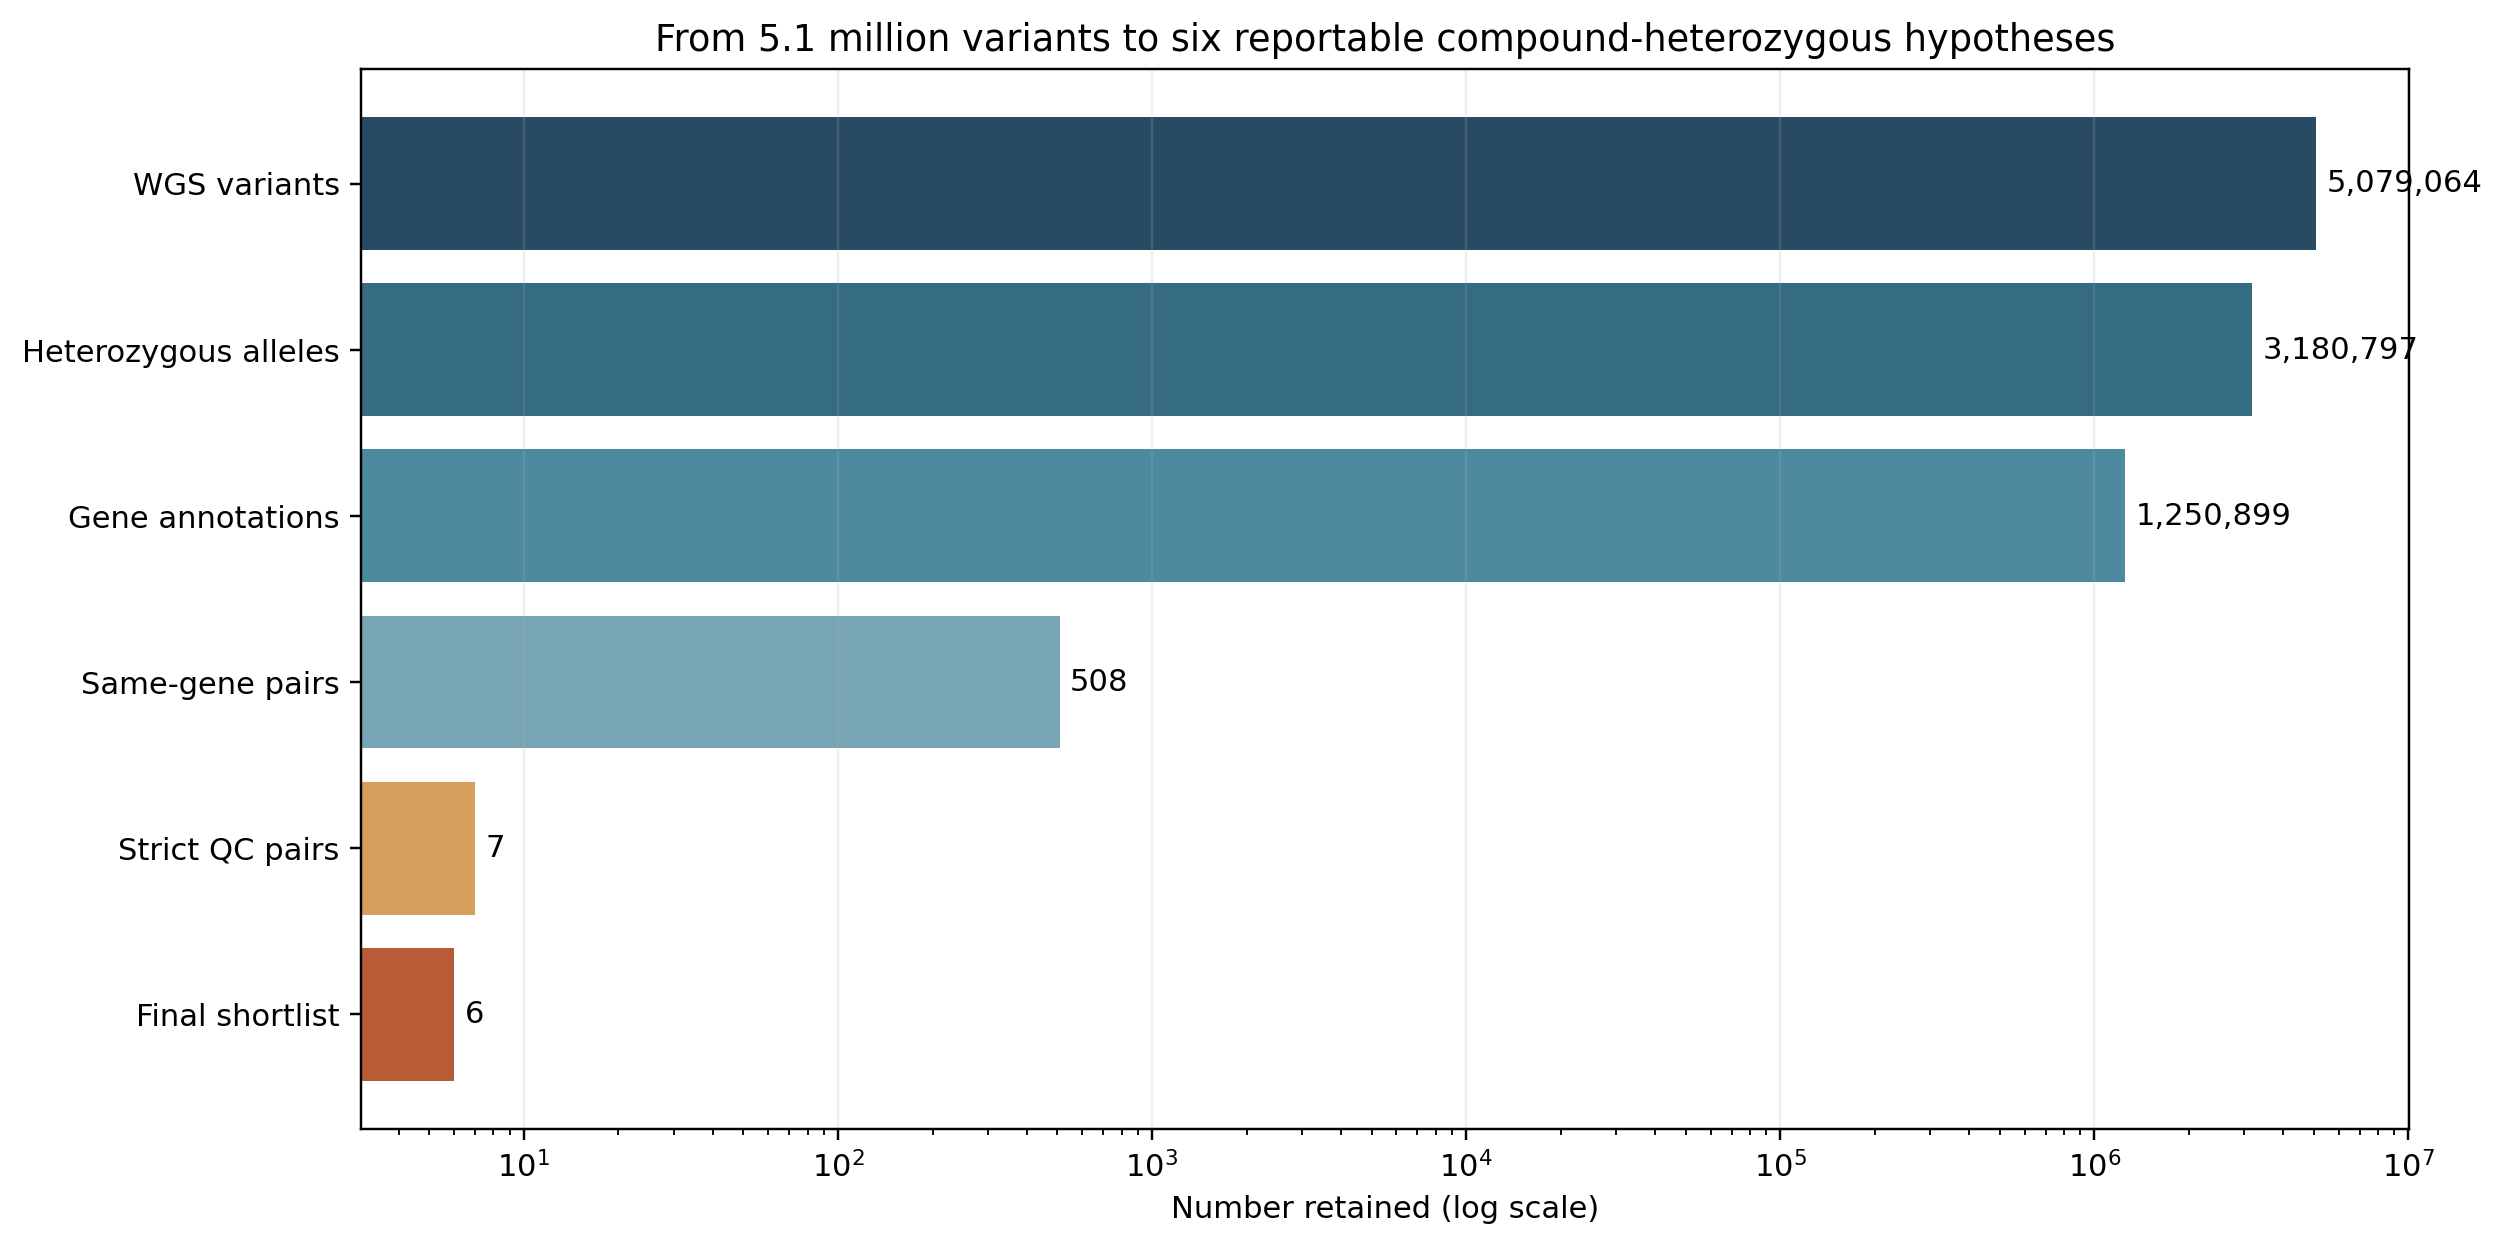
\includegraphics[width=0.94\textwidth]{figures/analysis_funnel.png}
\caption{The filtering funnel. Counts represent different objects at different stages: raw variants, heterozygous alleles, transcript/gene annotations, and finally genotype hypotheses. The logarithmic axis prevents the final six pairs from disappearing visually.}
\label{fig:funnel}
\end{figure}


\section{The goal of Bayesian Modeling}

The deterministic workflow already solved the child. A learned model is justified only if it adds knowledge beyond that case. We therefore separated three objectives:
\begin{enumerate}
\item \textbf{Track 1 compatibility:} preserve the accepted pair at rank 1.
\item \textbf{Molecular generalization:} recognize pathogenic variants that entered ClinVar after training.
\item \textbf{Patient generalization and uncertainty:} rank causal hypotheses for other solved diseases and identify unsupported cases.
\end{enumerate}

This changed the learning target. The model does not consume FASTQ reads. It receives annotated candidate alleles or pairs and predicts a pathogenicity or causality score. Deterministic processing remains responsible for valid observations and inheritance-consistent hypotheses.
\section{Model family 1: Bayesian conditional-logit pair ranker}

\subsection{Training data and target}

The first learned benchmark loaded 9,739 solved Phenopacket cases, including 959 reported two-variant cases. After annotation and decoy requirements, 425 cases were used for training, 44 for validation, and 89 for development testing. Genes, source publications, and case identifiers were disjoint across splits. \textit{BUB1B} was excluded.

Each case had 23 constructed candidate pairs. The target $y_i$ was the index of the reported causal pair. For feature vector $x_{ij}$ of candidate $j$ in case $i$, conditional logit assigns
\begin{equation}
p(y_i=j\mid X_i,w)=\frac{\exp(w^\top x_{ij})}{\sum_k\exp(w^\top x_{ik})}.
\end{equation}
A zero-centered Gaussian prior regularizes $w$. The maximum-a-posteriori estimate was optimized, and a Laplace approximation around it provided a Gaussian posterior. Prior scale was selected by validation negative log likelihood.

\subsection{Result}

On 89 held-out development cases, the fixed evidence rule achieved 70.8\% top-1 and 83.1\% top-5. The Bayesian posterior mean achieved 58.4\% top-1 and 87.6\% top-5. The learned model improved shortlist retention but was worse at rank 1. The negative result showed that 425 simplified cases were insufficient for an end-to-end pair learner to replace explicit biological structure.

\section{Model family 2: first low-rank SBNN pair model}

The first SBNN \citep{toure2026} used the same 15 pair features and 425/44/89 split. Its hidden widths were 32 and 16, with factor ranks $(8,8,1)$. For a Bayesian layer, a sampled weight matrix is represented by low-rank factors
\begin{equation}
W=AB^\top,\qquad q(A)q(B)q(b)=\prod_r\mathcal{N}(\mu_r,\sigma_r^2).
\end{equation}
Training minimizes a Monte Carlo estimate of
\begin{equation}
\mathcal{L}=\mathbb{E}_{q(W)}[-\log p(y\mid X,W)]+\lambda\,\mathrm{KL}[q(W)\Vert p(W)].
\end{equation}
Both random and SVD-based mean initialization were tested. Posterior predictive probabilities average softmax predictions over sampled weights. Mutual information between the sampled predictions and their mean estimates epistemic uncertainty.

The SBNN achieved 56.2\% top-1 and 87.6\% top-5 on the same development set. The result did not justify replacing the rule. It motivated a larger and cleaner variant-level task.

\section{Temporal ClinVar experiment}

\subsection{Why a temporal split}

Random ClinVar splits leak stable gene and annotation patterns. A temporal split asks a more useful question: can a model trained on the 26 December 2023 knowledge state classify records whose Variation IDs were absent then and appeared by 29 August 2026? Archived ClinVar releases make this test reproducible \citep{clinvar}.

The historical release supplied 1,084,930 unambiguous benign/pathogenic labels. A balanced 60,000-variant training set contained 30,000 pathogenic variants across 5,043 genes. A 15,000-variant gene-disjoint validation set contained 1,209 genes. The temporal test contained 626,287 new records, including 117,147 pathogenic variants across 14,715 genes.
\subsection{Fifty molecular features}

No clinical-significance label or disease name was used as an input. Features included reference/alternate length, variant type, transition status, substitution class, population frequency and missingness, dbSNP availability, germline/inherited/de-novo origin flags, review-level indicators, molecular consequence categories, and three gene-history quantities computed only from the training split: training count, pathogenic rate, and an unseen-gene flag.

\subsection{Core baselines}

Four aligned models used the same data and features:
\begin{itemize}
\item histogram gradient boosting, a strong nonlinear tabular baseline;
\item a dense 50-32-16-1 MLP;
\item a five-member independently trained MLP ensemble \citep{lakshminarayanan2017};
\item a low-rank SBNN with ranks $(8,8,1)$ \citep{toure2026}.
\end{itemize}
The temporal set was then split by ClinVar Variation-ID parity. Even IDs selected a consensus weight; 313,171 odd IDs remained untouched. The selected consensus was $0.30$ gradient boost, $0.20$ deep ensemble, and $0.50$ SBNN.
\begin{figure}[H]
\centering
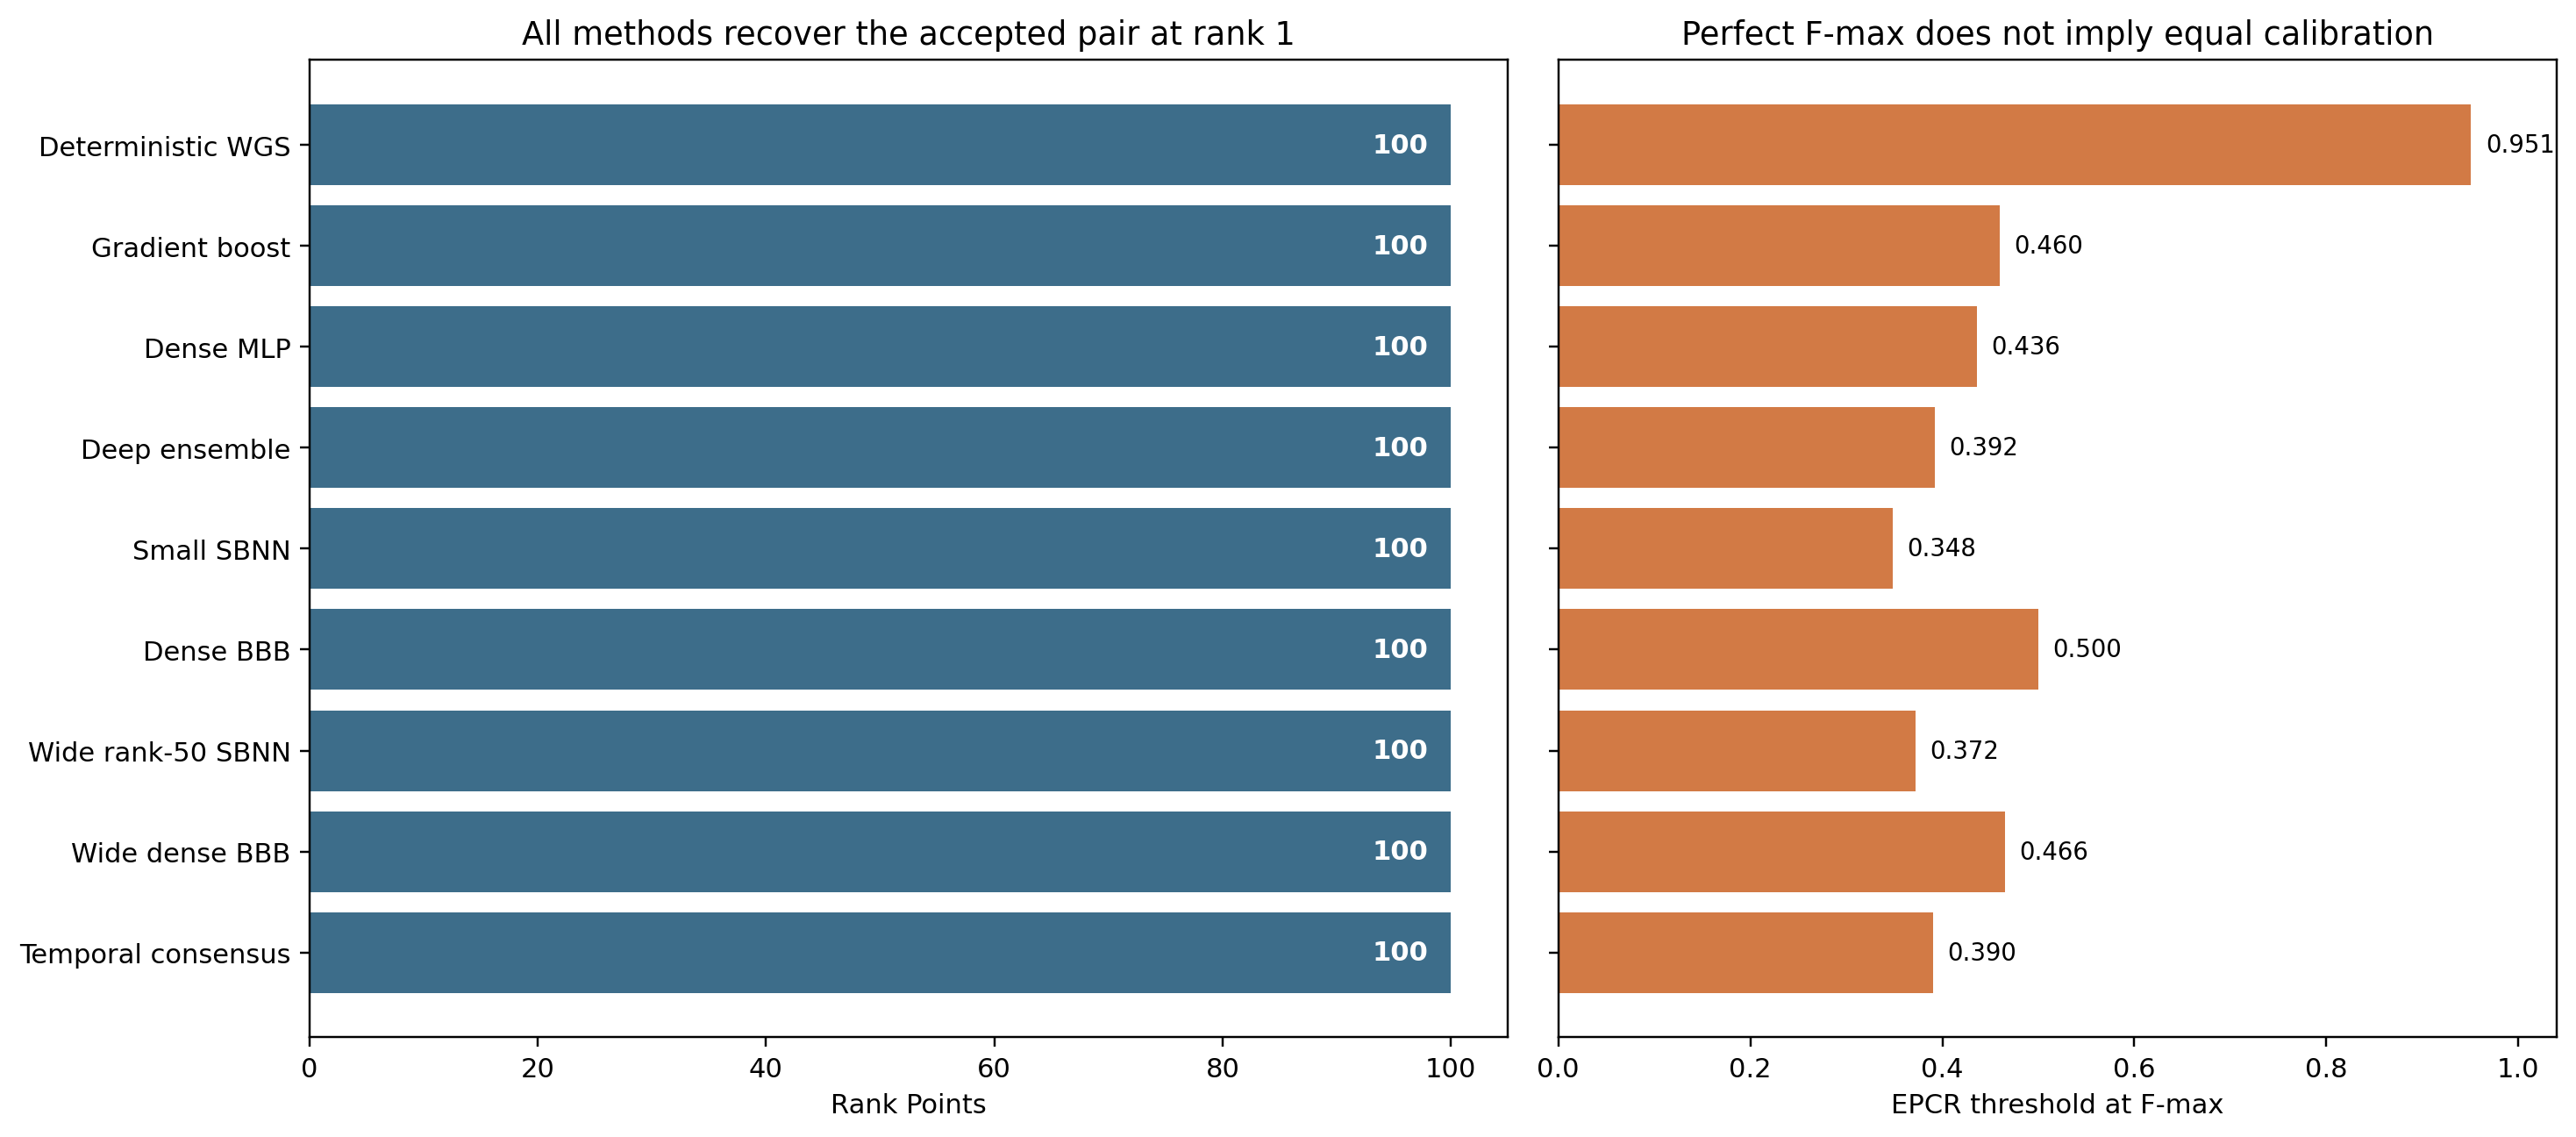
\includegraphics[width=\textwidth]{figures/track1_scores.png}
\caption{Every transferred model places the accepted pair first, but the EPCR threshold that isolates it varies widely. A perfect F-max on one child is not a calibration comparison.}
\label{fig:track1}
\end{figure}

The pair remains first because the upstream candidate construction is already strong: only biologically plausible same-gene pairs survive, direct cis evidence is removed, the \textit{BUB1B} pair combines a pathogenic stop-gain with an ultra-rare coding partner, and its phenotype score is high. The learned models order this compact set consistently. This is reassuring for robustness but cannot identify the best generalizing model.

\section{Temporal molecular results}

\begin{table}[H]
\centering
\caption{Untouched odd-ID temporal holdout. Ranking cases contain one pathogenic variant and 99 temporal benign variants.}
\small
\begin{tabular}{lrrrrrr}
\toprule
Model & PR-AUC & F-max & NLL & Top-1 & Top-5 & OOD AUROC \\
\midrule
Gradient boost & 0.9674 & 0.9030 & 0.1924 & 81.50\% & 94.05\% & -- \\
Deep ensemble & 0.9688 & 0.9095 & \textbf{0.1245} & 80.25\% & 95.00\% & \textbf{0.7485} \\
Small SBNN & 0.9691 & 0.9173 & 0.1332 & 82.10\% & 94.30\% & 0.6020$^*$ \\
Consensus & 0.9731 & 0.9181 & 0.1358 & 83.65\% & 94.80\% & -- \\
Dense BBB & 0.9729 & 0.9202 & 0.1245 & 83.00\% & 94.55\% & 0.6665 \\
Wide rank-50 SBNN & \textbf{0.9736} & \textbf{0.9235} & 0.1232 & \textbf{84.35\%} & 94.85\% & 0.6284 \\
Wide dense BBB & 0.9718 & 0.9200 & 0.1276 & 81.35\% & \textbf{95.05\%} & 0.6567 \\
\bottomrule
\end{tabular}
\begin{flushleft}\footnotesize $^*$The original small-SBNN OOD result was computed on the full temporal set; it is context rather than a perfectly matched holdout value.\end{flushleft}
\end{table}

\section{Bayesian architecture experiments}

\subsection{Factorial SBNN sweep}

We tested the interaction between rank, KL weight, posterior scale initialization, and broad prior scale rather than changing one variable at a time. The full grid contained 375 configurations:
\begin{itemize}
\item ranks $(8,4,1)$, $(8,8,1)$, $(16,8,1)$, $(16,16,1)$, and $(32,16,1)$;
\item KL weights $0.001$, $0.01$, $0.1$, $1$, and $3$;
\item posterior scale multipliers $0.1$, $0.3$, $1$, $3$, and $10$;
\item broad prior standard deviations $0.3$, $1$, and $3$.
\end{itemize}

The best confirmed compact configuration used ranks $(8,4,1)$, KL 0.01, posterior multiplier 0.1, and prior scale 0.3. Its unseen-gene OOD AUROC was 0.6231, up from 0.6020, but below the deep ensemble's 0.7485. Some screen configurations exceeded 0.70 OOD AUROC only by degrading classification toward chance. These were rejected rather than promoted as uncertainty improvements.

\subsection{Full-weight Bayes by Backprop}

The low-rank posterior couples uncertainty through $A$ and $B$. A dense BBB model instead assigns every weight and bias an independent Gaussian mean and rho \citep{blundell2015}. A 75-cell grid crossed rho initialization $\{-8,-6,-5,-4,-3\}$, KL weight $\{0.001,0.01,0.1,1,3\}$, and prior scale $\{0.3,1,3\}$. The winner used rho $-4$, KL 0.1, and prior scale 0.3.

Dense BBB used 4,354 variational scalars, versus 10,885 fitted weights across the five-network ensemble. On the untouched holdout it achieved 83.0\% top-1, F-max 0.9202, and OOD AUROC 0.6665. It improved ranking over the ensemble but did not match ensemble OOD detection.

\subsection{Wider low-rank and dense models}

To test whether the original network was simply too small, widths increased from 32-16 to 200-100. Ranks 8, 16, 32, 50, and the algebraically full factorization were crossed with KL and posterior-scale settings. The selected rank-50 SBNN used 55,804 variational scalars, only 8\% fewer than the matching wide dense BBB. It achieved the best temporal top-1 (84.35\%), PR-AUC (0.9736), F-max (0.9235), and 80\%-coverage balanced accuracy (99.12\%). Its OOD AUROC remained 0.6284.

This is an important result: increasing rank and width improved the main classification task but did not create ensemble-like function-space diversity.

\section{Track 1 comparison: every compatible model finds the pair}

The official evaluator logic was reproduced locally against the leaderboard-confirmed accepted pair. The deterministic CSV is the artifact actually uploaded and independently confirmed by the leaderboard. The learned CSVs were scored locally using the same logic.

\begin{longtable}{p{0.27\textwidth}rrrrp{0.24\textwidth}}
\caption{Exact child-level results.}\\
\toprule
Method & Rows & Pair rank & Rank Points & F-max & Status \\
\midrule
\endfirsthead
\toprule
Method & Rows & Pair rank & Rank Points & F-max & Status \\
\midrule
\endhead
Bonaventure deterministic WGS & 6 & 1 & 100 & 1.000 & Uploaded and leaderboard-confirmed \\
Linear Bayesian, strict & 6 & 1 & 100 & 1.000 & Local official-equivalent score \\
Linear Bayesian, broad & 10 & 1 & 100 & 1.000 & Local official-equivalent score \\
Pair SBNN, strict & 6 & 1 & 100 & 1.000 & Local official-equivalent score \\
Pair SBNN, broad & 10 & 1 & 100 & 1.000 & Local official-equivalent score \\
Gradient boost adapter & 6 & 1 & 100 & 1.000 & Local official-equivalent score \\
Dense MLP adapter & 6 & 1 & 100 & 1.000 & Local official-equivalent score \\
Deep ensemble adapter & 6 & 1 & 100 & 1.000 & Local official-equivalent score \\
Small SBNN adapter & 6 & 1 & 100 & 1.000 & Local official-equivalent score \\
Dense BBB adapter & 6 & 1 & 100 & 1.000 & Local official-equivalent score \\
Wide rank-50 SBNN adapter & 6 & 1 & 100 & 1.000 & Local official-equivalent score \\
Wide dense BBB adapter & 6 & 1 & 100 & 1.000 & Local official-equivalent score \\
Temporal consensus adapter & 6 & 1 & 100 & 1.000 & Local official-equivalent score \\
\bottomrule
\end{longtable}
\subsection{Result Analysis}

Every entry in the table uses the same 50 molecular features and the same untouched odd-ID test cases. For the ranking columns, 2,000 pathogenic temporal variants were each placed among 99 benign temporal variants sampled with a fixed seed. Top-1 and top-5 report where the known pathogenic item appears in that 100-candidate list. PR-AUC and F-max are calculated over all 313,171 odd-ID records. NLL evaluates probability quality and penalizes confident errors. OOD AUROC asks whether a model-specific uncertainty score can distinguish variants in genes absent from the 2023 training set; it is not another pathogenicity score. The consensus weights were chosen on even Variation IDs before the odd-ID table was evaluated.

\textbf{Gradient boosting} is the strong non-Bayesian tabular baseline. Its 81.5\% top-1 and 0.9674 PR-AUC show that much of the signal is already present in the engineered molecular features. It has no posterior or independently trained members, so we do not assign it a stochastic OOD score.

\textbf{The five-network ensemble} averages five dense networks trained independently from different initial conditions. Its top-1 result, 80.25\%, is not the best ranking result, but its NLL of 0.1245 and unseen-gene AUROC of 0.7485 are the strongest tested calibration and OOD combination. The disagreement is useful because independently optimized networks reach different function-space solutions.

\textbf{The original small SBNN} replaces deterministic dense layers with low-rank Gaussian factors and averages Monte Carlo weight samples. It improves top-1 to 82.1\%, but its 0.602 OOD AUROC is weak. This negative result is why rank, width, posterior initialization, prior scale, and KL weight were studied jointly rather than assuming that a Bayesian label guarantees useful uncertainty.

\textbf{The temporal consensus} combines gradient boosting, the ensemble, and the small SBNN using weights selected on the even-ID partition. It raises top-1 to 83.65\% and PR-AUC to 0.9731. This is evidence that their errors are complementary, although its score is a predictive mixture rather than a single coherent posterior.

\textbf{Dense BBB} assigns an independent Gaussian mean and scale to every network parameter. Its 83.0\% top-1, 0.9729 PR-AUC, and 0.6665 OOD AUROC improve on the small SBNN's ranking and OOD behavior. It still does not match the ensemble's unseen-gene detection.

\textbf{The wide rank-50 SBNN} uses 200- and 100-unit hidden layers and much less restrictive factors. It gives the best tested ranking: 84.35\% top-1, PR-AUC 0.9736, and F-max 0.9235. Its OOD AUROC remains 0.6284, so the result supports the larger SBNN as a pathogenicity ranker, not as the final uncertainty gate.

\textbf{The wide dense BBB} is the matching full-weight Bayesian comparison. It reaches 81.35\% top-1 and 0.6567 OOD AUROC, with the best top-5 value at 95.05\%. Widening alone therefore does not explain the rank-50 SBNN's top-1 gain, and a dense posterior does not automatically reproduce the ensemble's diversity.

\begin{figure}[H]
\centering
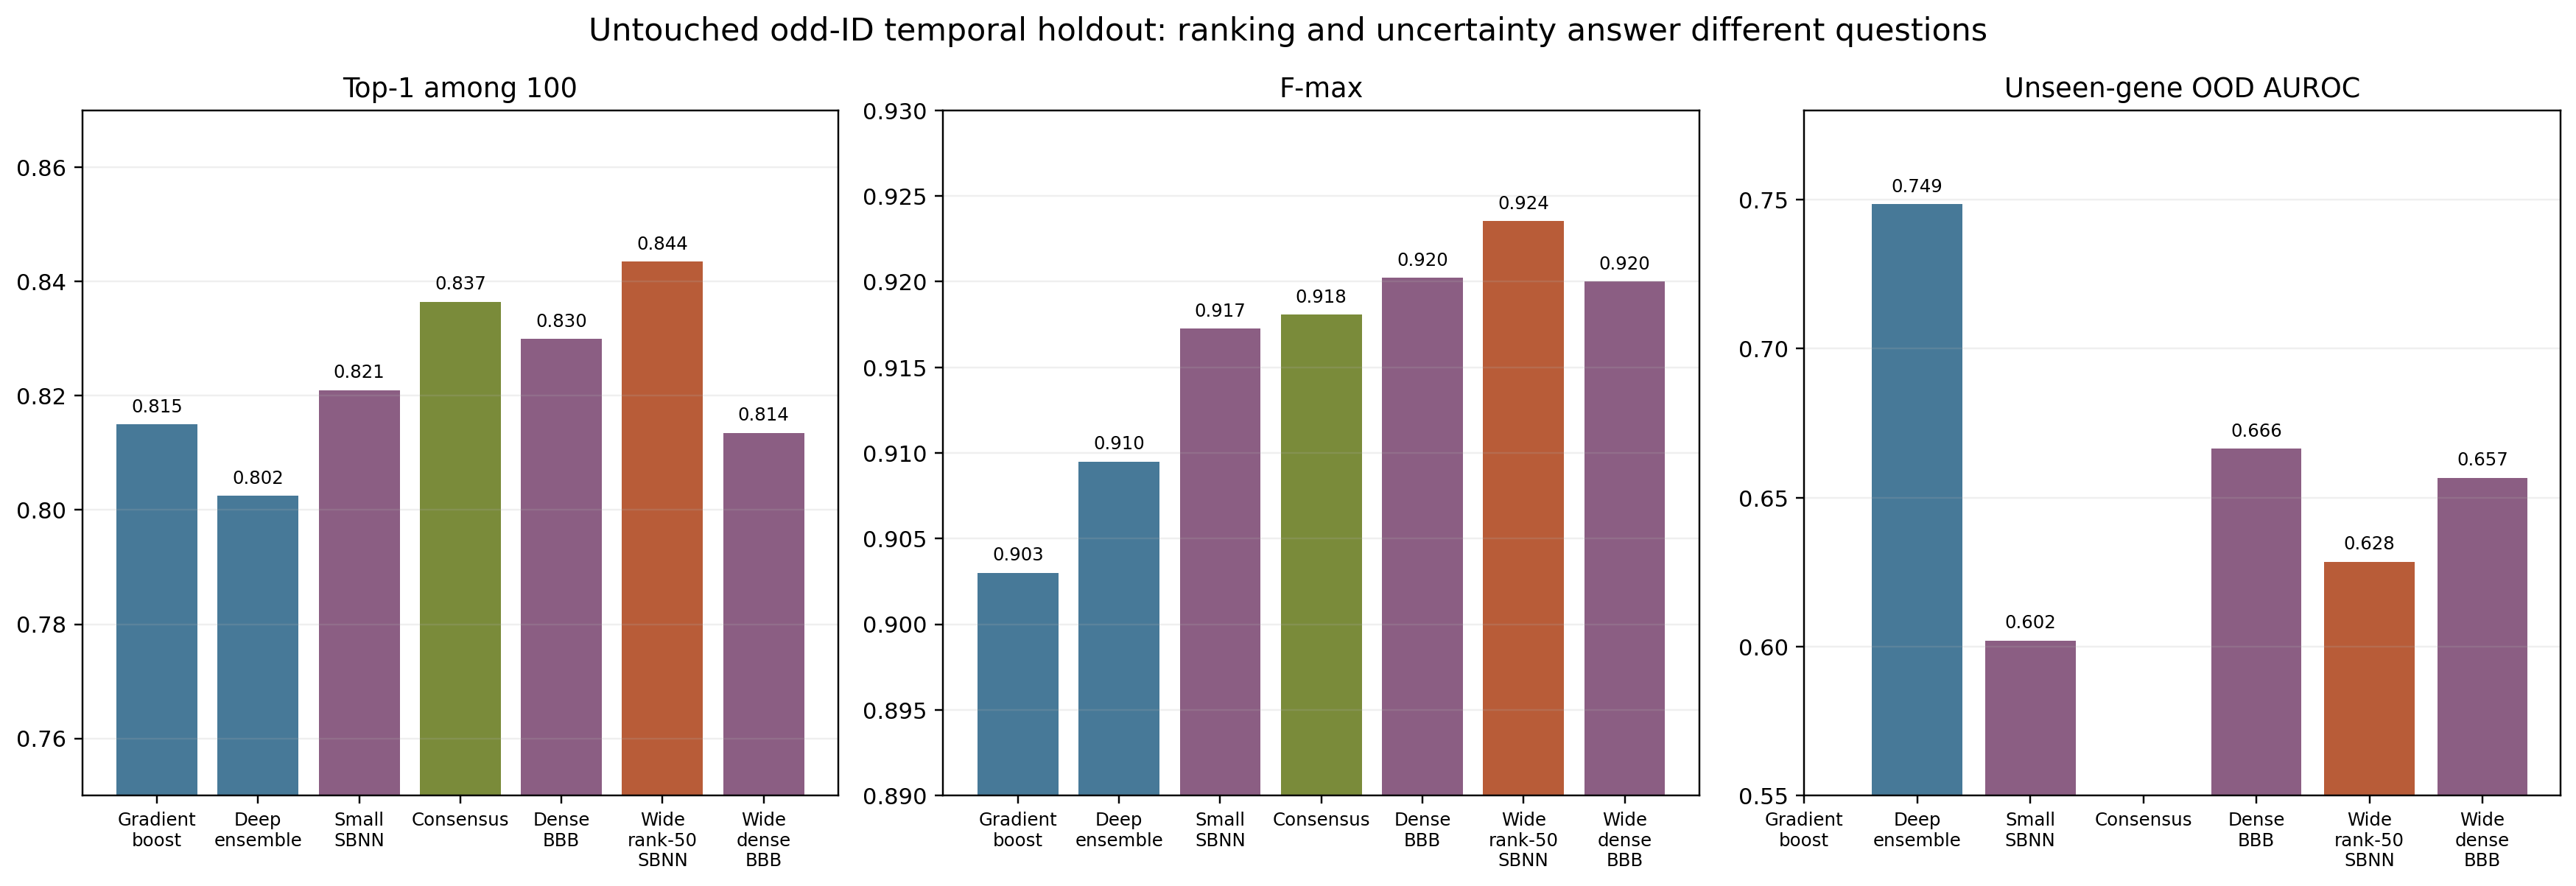
\includegraphics[width=\textwidth]{figures/temporal_model_comparison.png}
\caption{Task ranking, F-max, and unseen-gene detection favor different models. Empty OOD bars indicate that no model-specific stochastic uncertainty was defined for that method.}
\label{fig:temporal}
\end{figure}

\begin{figure}[H]
\centering
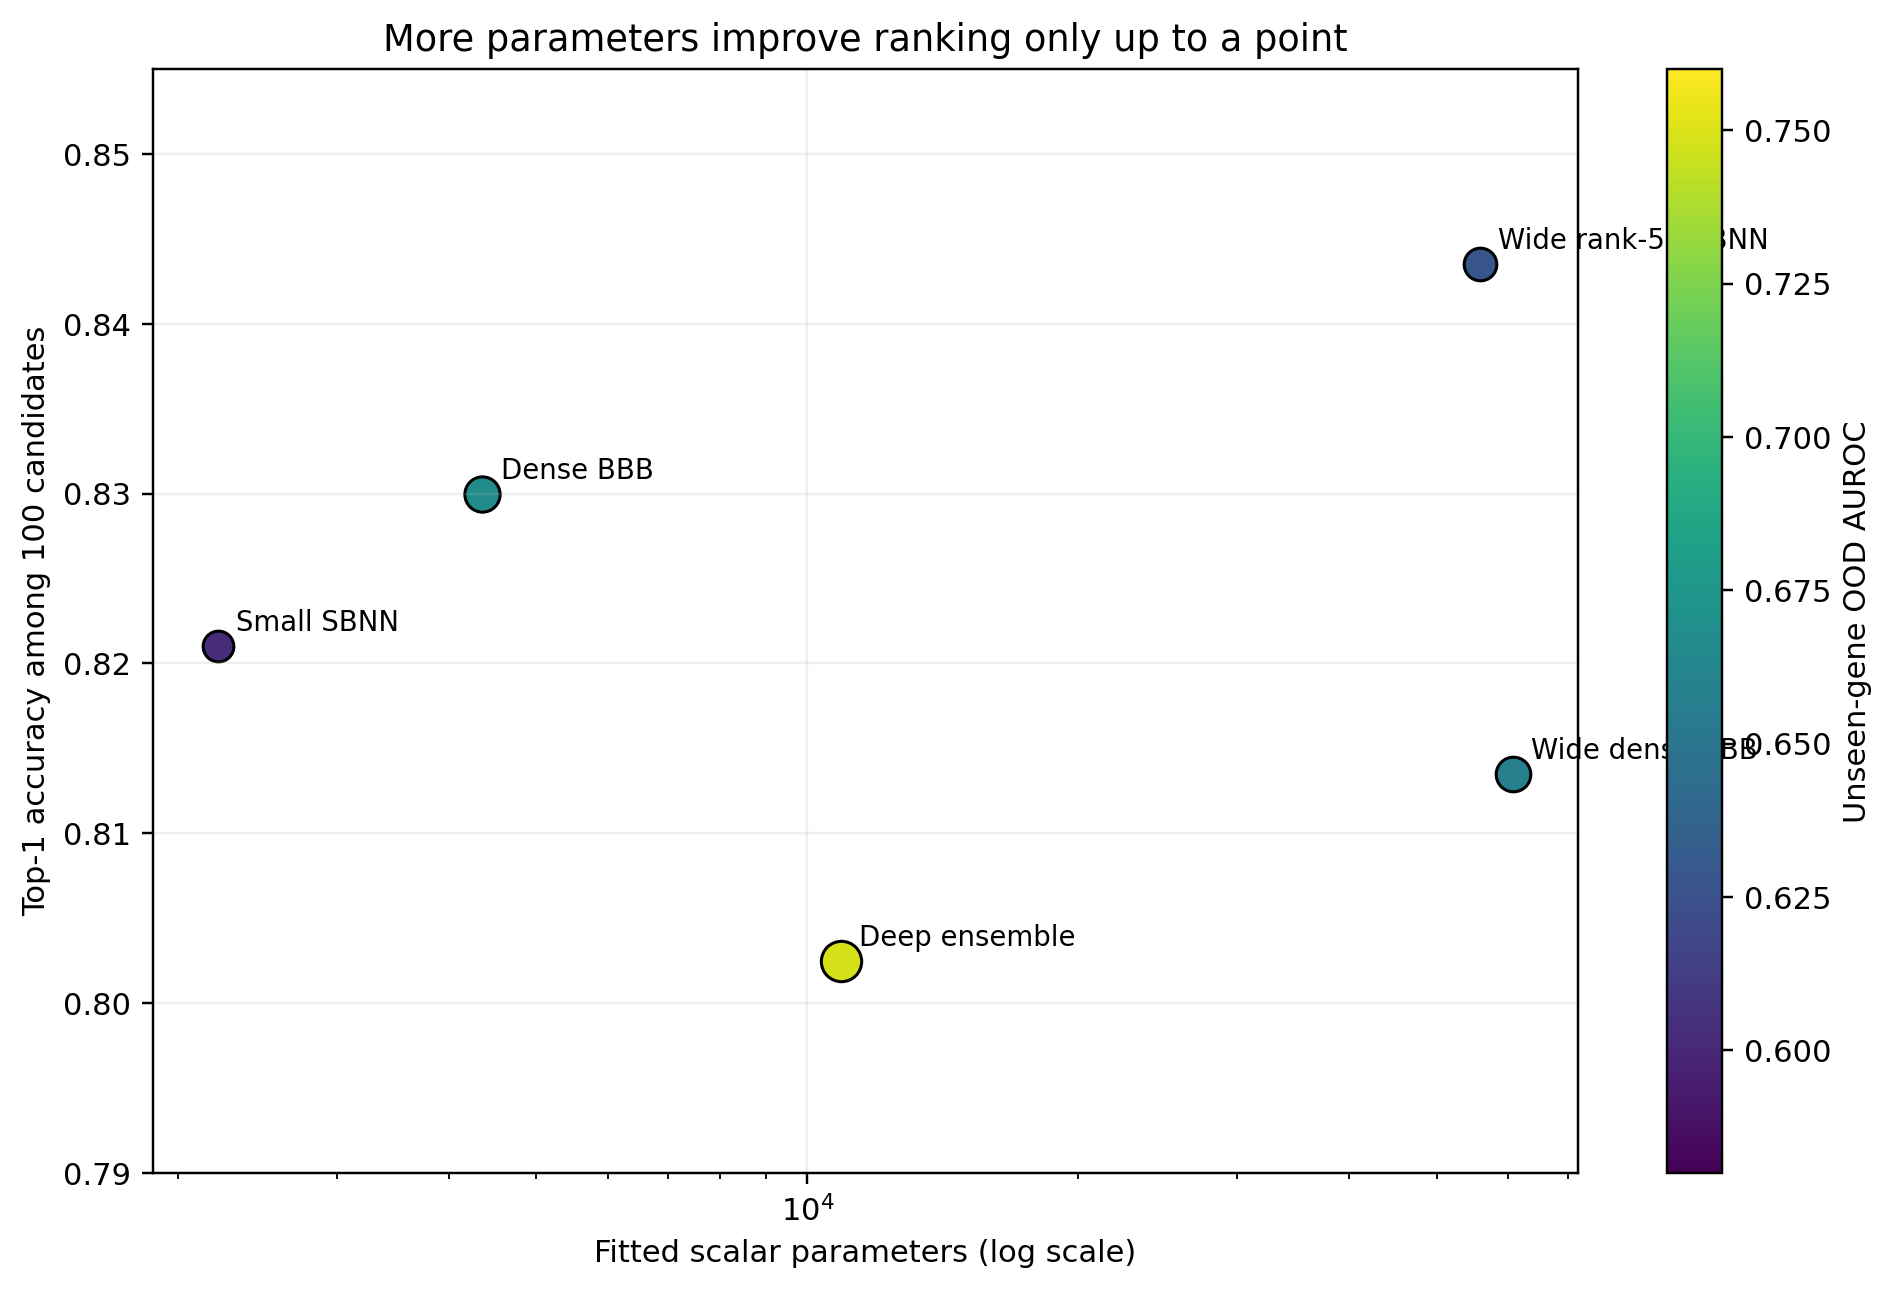
\includegraphics[width=0.82\textwidth]{figures/parameter_tradeoff.png}
\caption{Parameter count alone does not explain performance. The wide rank-50 SBNN gives the best ranking, while the smaller deep ensemble gives the strongest OOD signal because its members occupy independently optimized function-space modes.}
\label{fig:parameters}
\end{figure}
\section{External patient-level generalization}

\subsection{Construction without test leakage}

We next used Phenopacket Store cases with one or two exact GRCh38 causal variants. A causal hypothesis entered the test only when every causal coordinate was absent from the raw 2023 ClinVar snapshot and pathogenic in the 2026 snapshot. Repeated causal hypotheses were deduplicated. This retained 719 post-2023 cases from 265 genes: 655 single-variant and 64 two-variant cases.

Each case had one causal hypothesis and nine temporally new benign ClinVar hypotheses. Single-variant decoys were matched on variant type and consequence group when possible. Two-variant decoys contained two benign alleles in one gene. The molecular score of a pair was the geometric mean of its allele probabilities. Ten candidates imply a 10\% random top-1 baseline.

The HPO layer used only the 9 October 2023 ontology. Older solved cases were split into 1,388 phenotype-reference cases and 843 weight-selection cases. The validation split included familiar genes and genes entirely removed from the reference. For candidate gene $g$ and patient phenotype set $Q$, the score was the best symmetric Resnik similarity between $Q$ and an older case for $g$. Each model selected a molecular/HPO coefficient and missing-gene prior on the 843 older cases; the 719 post-2023 patients remained untouched.

Five independent benign candidate cohorts tested sensitivity to decoy composition. Reported means and sample standard deviations therefore reflect candidate resampling, not five independent patient cohorts.

\subsection{Results}

\begin{table}[H]
\centering
\caption{Mean top-1 generalization across five candidate cohorts.}
\small
\begin{tabular}{lrrrrr}
\toprule
Model & Molecular & Molecular+HPO & Change & HPO top-5 & Two-variant top-1 \\
\midrule
Gradient boost & 30.6$\pm$1.3 & 56.5$\pm$0.6 & +25.9 & 86.5 & 66.2 \\
Dense MLP & 29.2$\pm$0.8 & 55.9$\pm$2.0 & +26.6 & 84.3 & 65.9 \\
Deep ensemble & 30.6$\pm$0.7 & 54.2$\pm$1.9 & +23.6 & 85.0 & 64.1 \\
Small SBNN & 32.9$\pm$1.0 & 55.9$\pm$1.9 & +23.1 & 85.3 & 61.6 \\
Dense BBB & 34.1$\pm$1.0 & \textbf{58.9$\pm$1.0} & +24.8 & 88.5 & 65.6 \\
Wide rank-50 SBNN & 32.8$\pm$1.2 & 58.2$\pm$1.1 & +25.4 & 86.6 & 64.7 \\
Wide dense BBB & \textbf{34.2$\pm$1.4} & 58.6$\pm$1.4 & +24.4 & 85.9 & \textbf{68.1} \\
Temporal consensus & 34.0$\pm$0.5 & 57.3$\pm$1.7 & +23.3 & \textbf{88.6} & 64.4 \\
\bottomrule
\end{tabular}
\end{table}

\begin{figure}[H]
\centering
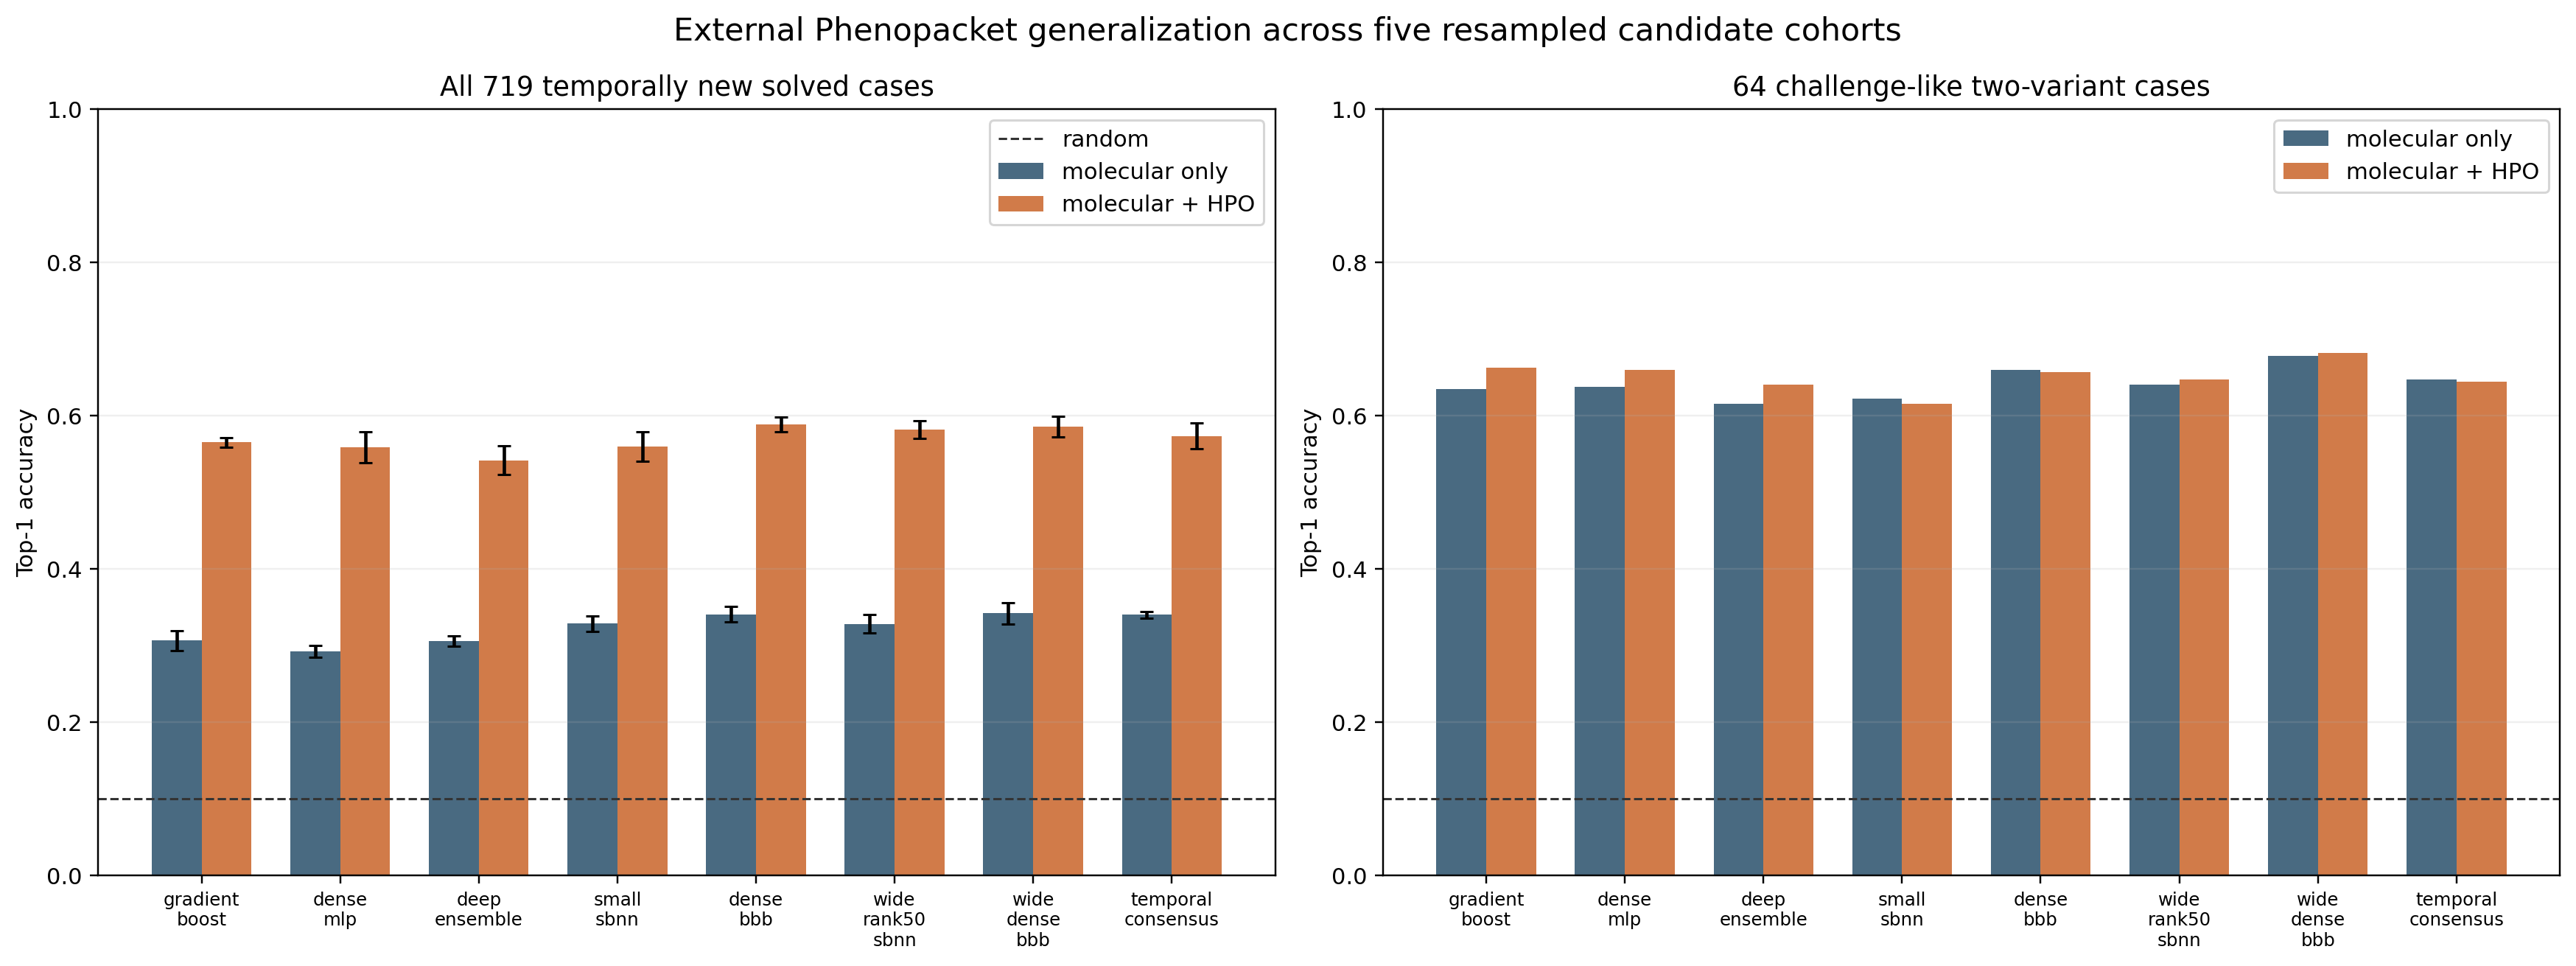
\includegraphics[width=\textwidth]{figures/external_generalization.png}
\caption{External patient-level ranking. Error bars in the left panel are standard deviations over five decoy cohorts. The two-variant subset is closest to the challenge's compound-heterozygous structure.}
\label{fig:external}
\end{figure}

For dense BBB, HPO conditioning improved top-1 accuracy by 23.5--26.1 \pp{} in every cohort. Each paired comparison gained 175--194 cases while losing only 2--6, with exact McNemar $p$-values between approximately $10^{-44}$ and $10^{-53}$. The effect is statistically clear within this benchmark.

\subsection{Known-gene and unseen-gene behavior}
Of the 719 test cases, 337 had a causal gene represented in older phenotype cases and 382 did not. Dense BBB rose from 34.7\% to 88.1\% top-1 on the known-gene subset, but stayed near baseline on unseen genes (33.6\% to 33.1\%). The tuned missing-gene prior prevents a catastrophic penalty when phenotype knowledge is absent, but it does not invent knowledge about novel genes.

\begin{figure}[H]
\centering
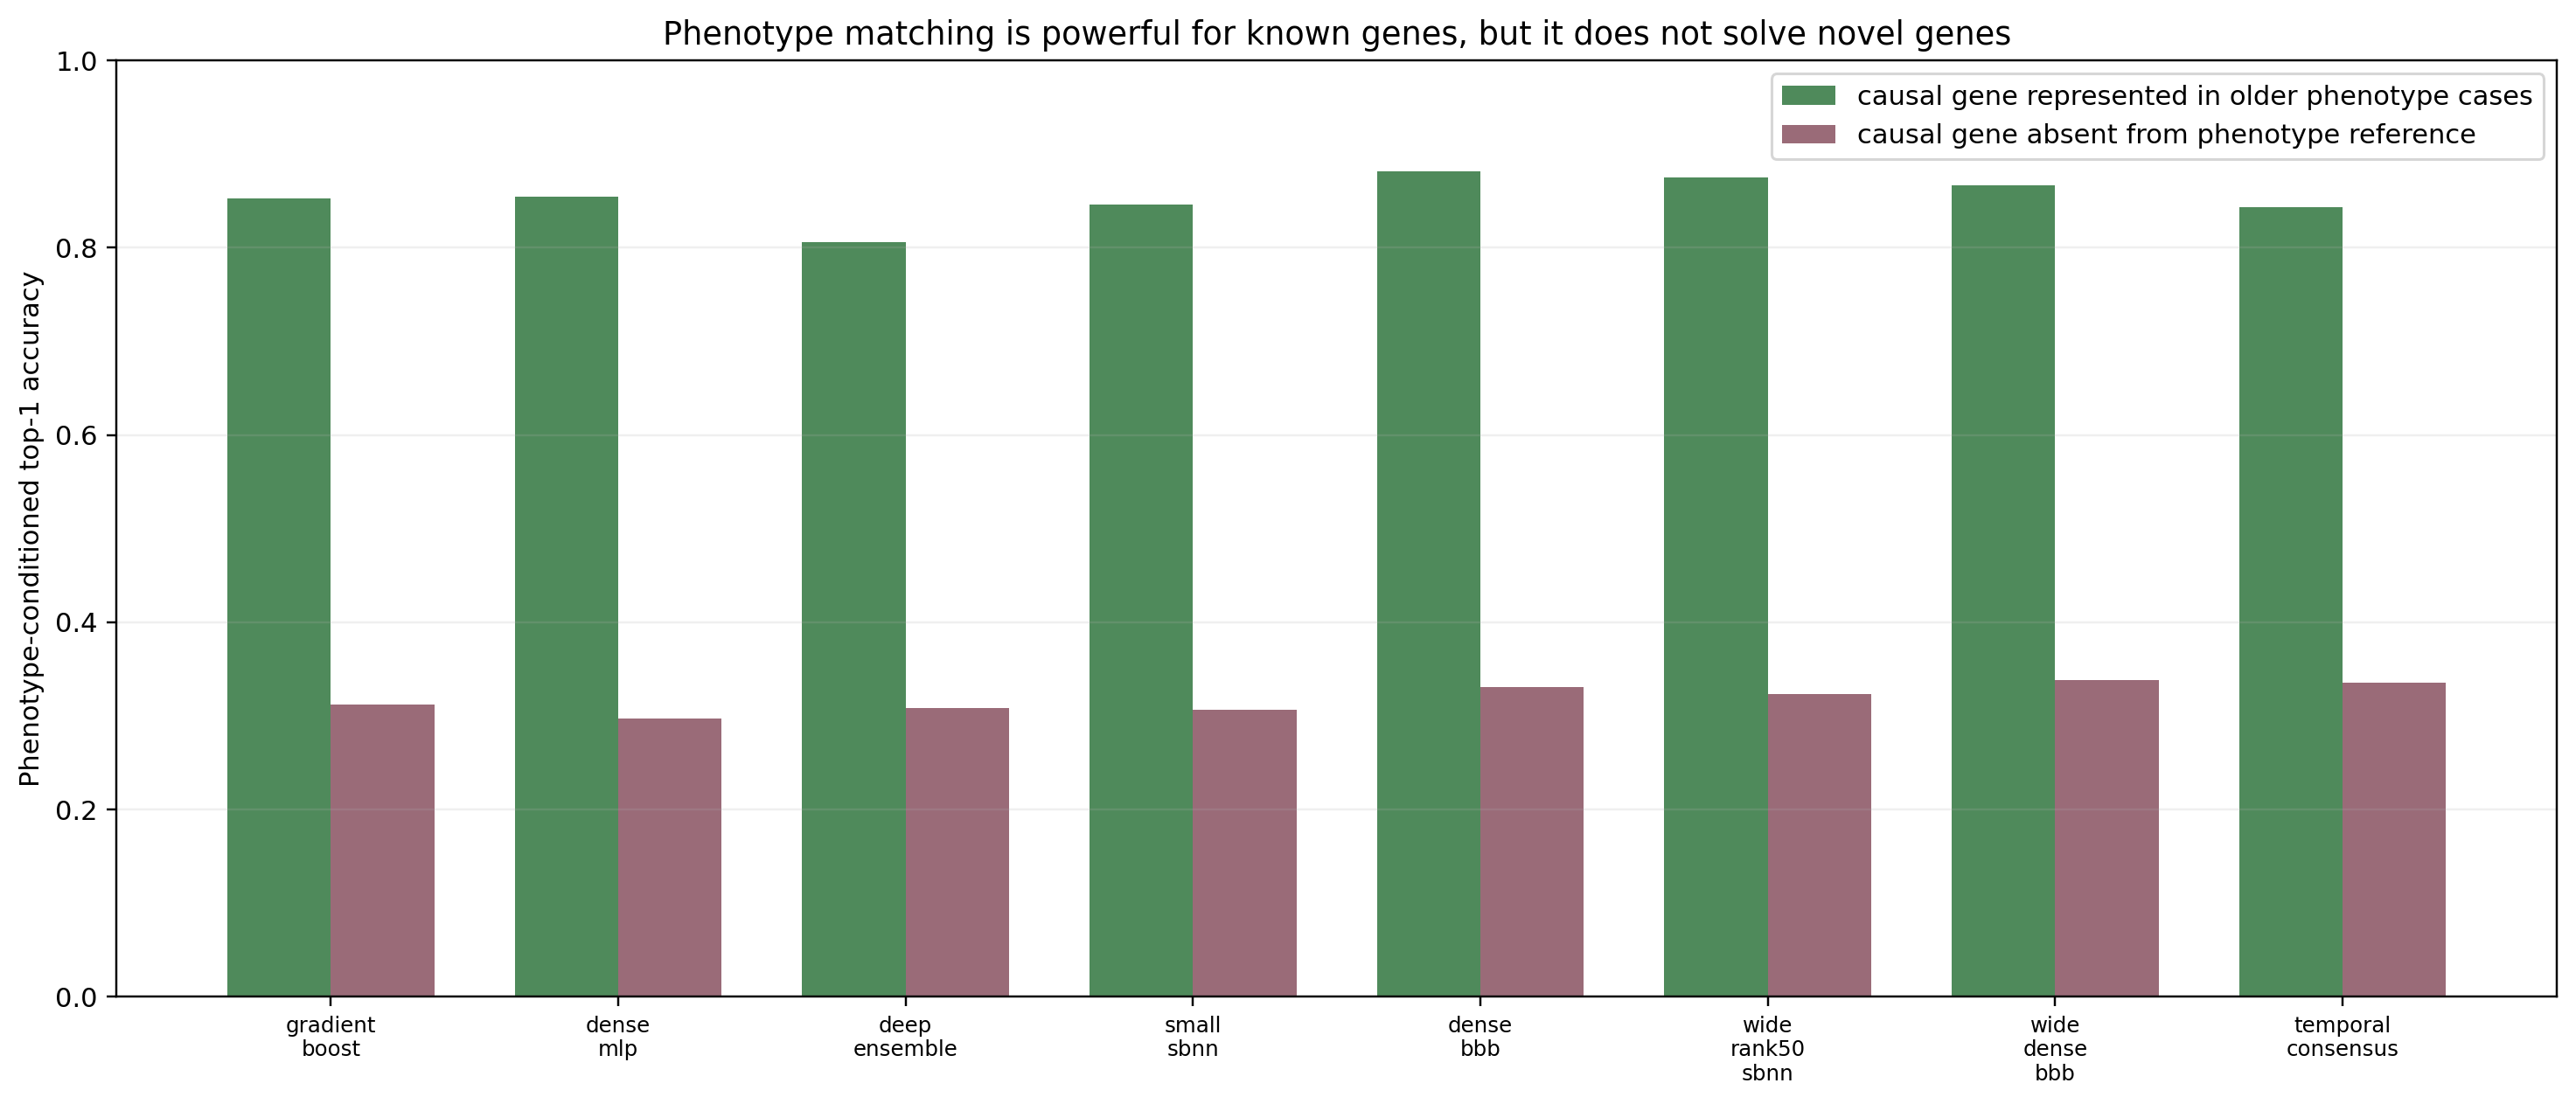
\includegraphics[width=0.92\textwidth]{figures/phenotype_coverage.png}
\caption{Phenotype matching works when the candidate gene has older phenotype evidence. Novel-gene diagnosis remains a molecular and discovery problem.}
\label{fig:coverage}
\end{figure}

\section{Calibration, uncertainty, and what Bayesian means here}

Three distinct probability concepts occur in the project:
\begin{enumerate}
\item the deterministic EPCR submitted for one child, a monotone ranking confidence;
\item posterior predictive probabilities from Bayesian weight distributions;
\item the clinical posterior probability of pathogenicity under ACMG/AMP evidence.
\end{enumerate}
They are not interchangeable. ACMG/AMP evidence can be expressed in Bayesian odds \citep{tavtigian2018}, but that does not make a neural posterior clinically calibrated.

For posterior samples $p_m(y\mid x)$, predictive entropy is
\begin{equation}
H\!\left[\bar p\right],\qquad \bar p=\frac{1}{M}\sum_{m=1}^M p_m,
\end{equation}
and epistemic mutual information is
\begin{equation}
I[y,W\mid x,D]=H[\bar p]-\frac{1}{M}\sum_{m=1}^M H[p_m].
\end{equation}
More Monte Carlo draws estimate the same posterior more accurately; they do not turn one narrow posterior into an ensemble of independently optimized modes.

This may explain the observed OOD gap. The tuned low-rank SBNN's mean predictive standard deviation rose from 0.00157 on known genes to 0.00403 on unseen genes. The deep ensemble rose from 0.01179 to 0.03569. Both react to shift, but the ensemble's function-space dispersion is roughly an order of magnitude larger. The honest conclusion is that the current Bayesian models improve several ranking and selective-prediction metrics, while the deterministic deep ensemble remains the strongest unseen-gene detector.
\section{How this compares with real rare-disease ML}

Production systems are hybrid. Exomiser combines frequency, predicted pathogenicity, pedigree, and phenotype evidence \citep{exomiser2015}. LIRICAL uses interpretable phenotype likelihood ratios with genotype information \citep{lirical2020}. MAVERICK trains on large variant datasets and adds structured inheritance reasoning \citep{maverick2023}. AI-MARRVEL trained a random forest on more than 3.5 million variants from diagnosed cases and combined learned predictions with expert-engineered features \citep{aimarrvel2024}. In the CAGI Rare Genomes Project, leading teams recovered up to 13 of 14 solved test families in their top five while still requiring clinical review \citep{stenton2024}.

Our design follows the same layered logic at smaller scale. The causal hypothesis must survive candidate generation before any ranker can score it. Molecular pathogenicity, phenotype compatibility, inheritance, phase, and read validity are distinct evidence sources. The Bayesian contribution is most defensible where uncertainty changes a decision: referral, abstention, reanalysis, or selection of an additional experiment.
\section{Summary of established results}

\subsection{Established by executed artifacts}
\begin{itemize}
\item The uploaded deterministic pipeline found the accepted \textit{BUB1B} pair at rank 1 and achieved Rank Points 100 and F-max 1.0.
\item Every compatible learned adapter also ranks the pair first under the locally reproduced official evaluator.
\item The temporal training corpus contains more than one million historical labeled variants and 626,287 new-ID test variants.
\item Wide rank-50 SBNN gives the best temporal simulated ranking and F-max among tested models.
\item Deep-ensemble disagreement is the best tested unseen-gene detector.
\item HPO conditioning selected only on older cases materially improves compact post-2023 patient ranking.
\item Tests, seeds, model artifacts, and metric JSON files are retained.
\end{itemize}

\subsection{Remaining gaps and next steps}
\begin{itemize}
\item The second \textit{BUB1B} allele has not been functionally proven pathogenic.
\item The two alleles have not been directly shown to be in trans.
\item The external 58.9\% result is not full-exome diagnostic sensitivity.
\item Candidate-generation recall has not been measured on an independent patient cohort.
\item The submitted EPCR is not clinically calibrated across patients.
\item No Bayesian model has beaten the deep ensemble on unseen-gene OOD detection.
\end{itemize}
\section{Track 2 bridge: from diagnosis to a testable rescue strategy}

The Track 1 mechanism suggests a Track 2 assay rather than an immediate drug claim. The p.Leu737Ter allele is loss of function. p.Asn1002Lys may affect BUBR1 abundance, localization, or kinase/checkpoint function, but this remains untested. The first experiment should therefore measure BUBR1 protein abundance and spindle-checkpoint function in patient-derived cells, with a CRISPR-corrected isogenic control and a \textit{BUB1B} add-back positive control.

A compound screen should measure BUBR1 abundance/localization, mitotic timing under spindle perturbation, lagging chromosomes, micronuclei, premature chromatid separation, viability, proliferation, and DNA-damage signals. A Bayesian hierarchical dose-response model can estimate the posterior probability of meaningful multi-endpoint rescue without unacceptable toxicity and choose follow-up compound-dose combinations by expected information gain.

The NAD+/SIRT2/BUBR1 stabilization axis is a mechanistic lead because SIRT2-mediated deacetylation can stabilize BUBR1 and NMN increased BUBR1 abundance in a mouse context \citep{sirt2bubr12014}. The balance among BUBR1, PP2A-B56, and Aurora B is another mechanistic control: loss of the BUBR1 pseudokinase domain reduces kinetochore PP2A-B56 recruitment and produces chromosome-alignment errors consistent with unbalanced Aurora B activity \citep{bubr1pp2a2020}. Neither study establishes an approved treatment for constitutional \textit{BUB1B} deficiency. A winning Track 2 proposal should preregister rescue and toxicity endpoints and reject compounds that only suppress proliferation or kill aneuploid cells.

\section{Reproducibility}

\subsection{Two computational environments}

The WGS pipeline and the later Bayesian experiments ran in different environments because they solve very different computational problems.

\textbf{Cluster WGS environment.} Bonaventure's pipeline \citep{dossourepo2026} ran in an existing pip environment, using CPU execution and six alignment threads. The memory-safe alignment settings were 2,000 read pairs per Python batch, 2,000,000 read pairs per process-isolated shard, and a 10,000,000-base BWA chunk. Sharding bounds worker memory; it does not downsample reads. The repository pins \code{pysam==0.24.0}; it also requires pybwa, WhatsHap, OpenCRAVAT, python-docx, openpyxl, certifi, pandas, NumPy, SciPy, and tqdm. The locally installed OpenCRAVAT resources observed during analysis were ClinVar 2026.07.01, gnomAD v2.1, gnomAD3 v3, REVEL v4.3a, SpliceAI v4.0, and CADD v1.6. Their combined storage requirement was about 160~GB.



\textbf{Bayesian ML and reporting environment.} Every temporal model evaluation, HPO generalization run, statistical aggregation, unit test, and report-specific plot in the integrated repository \citep{tourerepo2026} was executed on CPU on a MacBook Pro with an Apple M2 chip, 8 CPU cores (4 performance and 4 efficiency), 8~GB RAM, and macOS 15.2 arm64. No GPU, PyTorch, TensorFlow, or accelerator backend was used. Python was 3.12.7 from Anaconda, compiled with Clang 14.0.6. NumPy used OpenBLAS 0.3.21.

\begin{table}[H]
\centering
\caption{Exact local package versions.}
\begin{tabular}{ll@{\qquad}ll}
\toprule
Package & Version & Package & Version \\
\midrule
NumPy & 1.26.4 & SciPy & 1.13.1 \\
scikit-learn & 1.5.1 & Matplotlib & 3.9.2 \\
pandas & 2.2.2 & joblib & 1.4.2 \\
threadpoolctl & 3.5.0 & pytest & 7.4.4 \\
Pillow & 10.4.0 & huggingface-hub & 0.36.0 \\
\bottomrule
\end{tabular}
\end{table}

The pinned local environment is stored in \path{requirements-report.txt}. Running \texttt{python} \path{capture_environment.py} regenerates \path{report/environment_manifest.json}, including hardware, Python, package versions, and SHA-256 hashes for the compact public inputs.

\subsection{Randomness and numerical execution}

All temporal experiments use seed 20260905 unless an output records a different seed. The five patient-level candidate cohorts use seeds 20260905 through 20260909. Data partitions are deterministic: the first pair benchmark separates genes and source publications, the temporal consensus uses even Variation IDs for selection and odd IDs for holdout, and the post-2023 Phenopacket test is separated by exact coordinate absence from the 2023 ClinVar snapshot. Posterior draw counts are stored in each result JSON. The Track 1 linear Bayesian and pair-SBNN runs used 2,048 posterior draws; temporal experiments used the model-specific counts written to their experiment reports.

The implementations clip probabilities before logarithms, standardize features using training-only statistics, replace near-zero feature scales with one, and keep pair scoring symmetric through a geometric mean. These details avoid seed-dependent NaNs, division by zero, and allele-order artifacts.

\subsection{Code map}
The code map combines the imported genome-wide workflow with the Bayesian modeling, evaluation, and reporting modules maintained in the integrated repository \citep{dossourepo2026,tourerepo2026}.
\small
\begin{longtable}{p{0.38\textwidth}p{0.54\textwidth}}
\toprule
File & Role \\
\midrule
\path{mva_track1_pipeline.py} & Bonaventure's genome-wide processing, annotation, phenotype scoring, filtering, pair construction, and export. \\
\path{shared_pair_features.py} & Fifteen features shared by pair training and Track 1 inference. \\
\path{bayesian_pair_ranker.py} & Conditional-logit MAP fit and Laplace posterior. \\
\path{sbnn_pair_ranker.py} & Low-rank SBNN and dense BBB layers, posterior sampling, and KL terms. \\
\path{clinvar_temporal_experiment.py} & Temporal dataset parsing, 50-feature construction, baselines, ranking, calibration, and uncertainty. \\
\path{tune_sbnn_temporal.py} & Factorial SBNN hyperparameter sweep. \\
\path{full_bbb_temporal_experiment.py} & Dense Bayes-by-Backprop comparison. \\
\path{wide_rank_temporal_experiment.py} & Width and rank experiment. \\
\path{verify_temporal_models_track1.py} & Common Track 1 adapter and exact scoring audit for temporal models. \\
\path{phenopacket_hpo_generalization.py} & Leakage-controlled post-2023 patient benchmark with HPO conditioning. \\
\path{aggregate_hpo_generalization.py} & Five-seed aggregation and uncertainty summaries. \\
\path{report_visualizations.py} & Rebuilds every report-specific figure from JSON artifacts. \\
\bottomrule
\end{longtable}
\normalsize

\subsection{Rebuilding figures and PDF}
From the repository root:
\begin{lstlisting}[language=bash]
./build_report.sh
\end{lstlisting}
This one command captures the local environment, rebuilds the seven figures, runs all 24 unit tests, re-scores the stored Track 1 outputs, and compiles the cited PDF. It uses the retained model checkpoint and compact candidate archive; it neither downloads the 85~GB challenge bundle nor retrains the expensive models. The individual report commands are:
\begin{lstlisting}[language=bash]
python report_visualizations.py --output-dir report/figures
cd report
pdflatex main.tex
bibtex main
pdflatex main.tex
pdflatex main.tex
\end{lstlisting}

The unit suite is:
\begin{lstlisting}[language=bash]
python -m pytest test_sbnn_pair_ranker.py \
  test_bayesian_integration.py test_audit_submission.py \
  test_clinvar_temporal_experiment.py -q
\end{lstlisting}
\subsection{AI assistance disclosure}

Coding agent were used ot help with code implementaiton. All analyses, research decisions and results were completed by the team.

\section{Final interpretation}

The child's result is stable. A pathogenic \textit{BUB1B} stop-gain and an ultra-rare missense partner explain the MVA phenotype better than the retained alternatives, and the pair remains first under deterministic, linear Bayesian, ensemble, low-rank Bayesian, full-weight Bayesian, wide, consensus, and phenotype-conditioned scoring.

The perfect leaderboard score is the beginning of the argument, not the end. The evidence that distinguishes the submission is the genome-wide discovery without a manual disease-gene bonus, the nearly complete annotation join, conservative handling of phase and the uncertain second allele, exact attribution of upstream features, temporal training and holdout design, factorial Bayesian experiments, honest negative OOD results, and patient-level transfer across hundreds of later solved cases.

No one model wins every metric. The wide rank-50 SBNN is the strongest tested temporal ranker. Dense BBB is the strongest overall HPO-conditioned external model. Wide dense BBB is strongest on the challenge-like two-variant subset. The deep ensemble is the strongest OOD detector. The correct final system is modular: deterministic biological validity, learned molecular evidence, ontology-aware phenotype matching, explicit inheritance logic, and uncertainty used to decide when evidence is insufficient.

The next empirical milestone is a full patient-specific PhEval run \citep{pheval2025}. It should measure candidate-generation recall separately from ranking, preserve complete VCF backgrounds, and test seen versus unseen genes, phenotype corruption, and inheritance modes. That experiment would convert the current strong compact-benchmark evidence into a defensible end-to-end diagnostic generalization claim.

\appendix
\section{Feature definitions for the first pair models}

\small
\begin{longtable}{p{0.30\textwidth}p{0.62\textwidth}}
\toprule
Feature & Meaning \\
\midrule
\code{phenotype\_score} & Bonaventure pipeline's HPO-based compatibility between the patient's terms and the candidate gene. \\
\code{min/max\_consequence} & Weakest and strongest normalized consequence severity among the two alleles. The minimum matters because both alleles must plausibly damage a recessive gene. \\
\code{min/mean\_rarity} & Rarity evidence across the pair. A frequent second allele weakens a recessive hypothesis. \\
\code{max\_population\_af} & Largest observed AF among the two alleles. \\
\code{af\_observed\_fraction} & Fraction of alleles with a measured AF, separating missingness from a true zero. \\
\code{min/max\_cadd} & CADD PHRED divided by 40 and clipped to $[0,1]$. \\
\code{cadd\_observed\_fraction} & Whether zero means missing or measured. \\
\code{min/max\_spliceai} & SpliceAI delta evidence across alleles. \\
\code{spliceai\_observed\_fraction} & Availability of splice predictions. \\
\code{phenotype x min consequence} & Interaction requiring phenotype and both-allele molecular plausibility. \\
\code{phenotype x min rarity} & Interaction requiring phenotype and two rare alleles. \\
\bottomrule
\end{longtable}
\normalsize

\section{Metric definitions}

\begin{description}
\item[Top-$k$] Fraction of ranking cases whose causal item is among the first $k$ candidates.
\item[MRR] Mean reciprocal rank, $N^{-1}\sum_i 1/r_i$.
\item[PR-AUC] Area under precision-recall curve; emphasized because pathogenic variants are the minority in the temporal test.
\item[NLL] Negative log likelihood; penalizes confident wrong predictions.
\item[Brier score] Mean squared error of predicted probabilities.
\item[ECE] Expected calibration error over 15 bins; descriptive and bin-dependent.
\item[OOD AUROC] Ability of an uncertainty score to distinguish variants from genes unseen during training.
\item[Selective accuracy] Accuracy after retaining only the least-uncertain fraction of predictions.
\end{description}

\section{Public input checksums}
\begin{lstlisting}
510c54e3fd04b0786f0a110bab63853e9e8fc3e9dde9e07ce7bc83f10cb63786  clinvar_20231226.vcf.gz
e72f5619f003c80cb3051afcb0c1f11c4409741054b48bbfd0ced03046ec91f9  clinvar_20260829.vcf.gz
d0c70005bb09b87035087516252b6b539fbc0415be7c664b73c9cde7eedf205a  all_phenopackets_v0.1.27.zip
d3c1280f2780628cc2adc41d43ad92eab8fa4c2bab0f421e6334c7b1e6cd4e52  hp_2023-10-09.obo
\end{lstlisting}
\bibliographystyle{unsrtnat}
\bibliography{references}
\end{document}
